
\chapter{Microstructure and WDS Analysis of the X--X$_3$Si Alloys}

The aim of Wavelength Dispersive Spectrometry (WDS) analysis is to gather more reliable evidence in order to provide an explanation of microstructures seen.  Many of the alloys were initially assessed by optical microscopy and SEM/EDS.  This has been briefly described in the previous chapter.  It was difficult to interpret the EDS data collected, as there were too many uncertain factors to draw any worthwhile conclusions.

The WDS data was collected using five detectors that can each be assigned to collect several specific wavelength ranges corresponding to the waves emitted by an element.  Collected wavelength ranges can be selected such that any overlap of peaks from different elements is eliminated.  When performed correctly, accuracy of WDS data can be within a narrow range of 100 $\pm$0.1wt.\%.  

We present the binary and ternary alloys as a set in the first portion of this chapter, and the quaternary and quinary alloys as a set in the second portion.
%\ref{section:Microstructure of Quinary \ilovewill{山}WAl}. 
In current literature, only binary phase-diagrams of the binary alloys are available.  We seek to:

1.  Expand existing phase-diagram knowledge in the ternaries, quaternaries and quinaries explored in this project.

2.  Examine the extent to which solidified alloys reflect consistent equilibrium compositions, and demonstrate that  compositional variation within each ingot illustrate that mobility is very difficult across these systems.

The various microstructures presented in this Chapter will be summarised in Conclusions, together with any suitable mechanical data that can be used.

\section{Calibration, Set-up and Method of WDS Data Collection}

Prior to WDS analysis, simulations were run in simulation software ``Virtual WDS" to help determine the experimental set-up for optimal data acquisition.  This software allows us to avoid the majority of situations that produce results of poor quality by selecting the K, L and M lines of elements used such that they do not overlap and interfere with each other.  Empirical observation then allows us to modify the parameters of non-ideal data acquisition situations, but may not improve data quality.  

A 20nA beam was used to obtain better collection statistics and better minimum detection levels.  Frequent calibration using silicate and pure element standards ensured sound data, and only measurements that fell within 100.0$\pm$0.8 total weight percent were taken.  Peak profiles collected for each elemental standard were used to specify the range of wavelengths to be collected for each element in the alloys.  Ideally, the peaks with the strongest signal were chosen.  However, if any peak selected for collection overlapped with another, weaker peaks for the elements involved would have to be selected instead.  This would minimise data collection inaccuracies.  Overlap typically occurred with elements that are next to each other on the periodic table, such as tantalum and tungsten.  In order to obtain statistically reliable data, 10 seconds was spent collecting the background signal of each peak, and 20 seconds was spent collecting the signal from each peak.  Si has some overlap with Ta and W. 

A typical method for obtaining bulk eutectic compositions would be to get an area scan made up of adjacent line scans.  Large areas of 100-200\micro\square\metre\ could be analysed by having consecutive line scans performed within the selected region.  Such line-scans would make rapid passes along the selected area, spending micro-seconds at each point along the pass.  The line-analysis data collected would have inferior statistics to spot-analysis.  Alternatively, the WDS set-up could be configured such that the beam spot size is very large, with a diameter of 100\micro\metre.  The maximum diameter of beam striking the sample surface is controlled by the working distance between sample surface and where the beam is last influenced by the electromagnetic coils, and also the strength and range of the electromagnetic coils used to deflect the electron beam.  When performing WDS, working distance is typically standardised to 15 \centi\metre.  If working distance was increased to increase beam size on the sample surface, calibration will have to be performed at this working distance.  Regardless of whether a change of working distance is implemented, the beam striking the sample surface could thus be a lot smaller than 100\micro\metre\ and measuring it would be a protracted process.  It is difficult to determine the exact dimensions of the area being analysed when the diameter of the beam is set up to be overly large.  The alternative of increasing the working distance would involve recalibration of the WDS to the new working distance.  This process would be non-trivial, and was deemed unnecessary to pursue.

It was decided that the most sensible method to determine alloy mean compositions was to measure grids of 5x5 to 10x10 of large 10-20\micro\metre\ spots.  These grids make the data collected statistically random.  In alloys where insufficient eutectic area fraction translate to small regions of eutectic, grid analysis cannot be performed.  Instead, the spots had to be site specific to prevent any interference from dendrites.  The spots were large enough to cover a substantial area, but small enough to accurately determine the location and dimensions of the area analysed by each spot.  A large inter-spot distance was placed between spots to prevent any sample volume from being part of more than one analysis.  This distance of 15--50\micro\metre\ would scale with spot size, with the aim to minimise analysis of a volume that had already been compromised by the electron beam.  Averaging the results obtained, after removing outliers, would give an alloy’s average composition.  A microstructure may be eutectic on the sample surface, but there may be a dendrite of one phase lying right beneath the surface.  This would result in a distinctly non-eutectic composition, which would skew the average composition.  We will find that obtaining average compositions would oversimplify the data, and that it would be more illustrative to provide a composition range for each alloy. 

1\micro\metre\ spot analyses of the individual phases were performed only on the DS alloys, as the lamellar spacing of the non-DS alloys were too small to provide sufficient analysis volume for accurate measurements.  
The distribution of measured compositions has been shown in a composition map (Figure \ref{fig:ternarymap}).  The five alloys measured have compositions which span the full range between Cr--Cr$_3$Si and V--V$_3$Si, as in the case of Figure \ref{fig:WDSaveragecompo}.  These plots reflect tie-lines in the phase-diagram.  All alloys followed the same trend of having an X$_3$Si phase with 19--23 at.\% Si, and a solid-solution phase. The bulk eutectic compositions lie between 9--16at.\%Si.  
Why is there a large range of 3-10at.\% Si in measured bulk eutectic compositions? Melts that deviate slightly from eutectic composition are guided down a solidification trough to the eutectic point, where the rest of the alloy solidifies at a specific composition.  The following is a summary of possible explanations:

Case 1.
There may be dendrites present very near the analysed surfaces due to the difficulties in achieving alloy manufacture of high quality, where homogeneous ingots would comprise of at least 95\% volume fraction of lamellar microstructure.  Instead, rampant dendritic growth was present in the majority of alloys explored.  Alloys systems in which dendritic growth could be curtailed are \ilovewill{山}W, \ilovewill{山}WAl.  Dendrites, being composed of one phase only, would skew the collected data away from the euctectic composition, and towards its composition.  This leads to a larger range of compositions measured even if the eutectic microstructure has a very narrow composition range.  Unfortunately, minimising the occurrence of dendrites was very difficult with the routes of manufacture pursued in this project.

%
\begin{figure}[H]
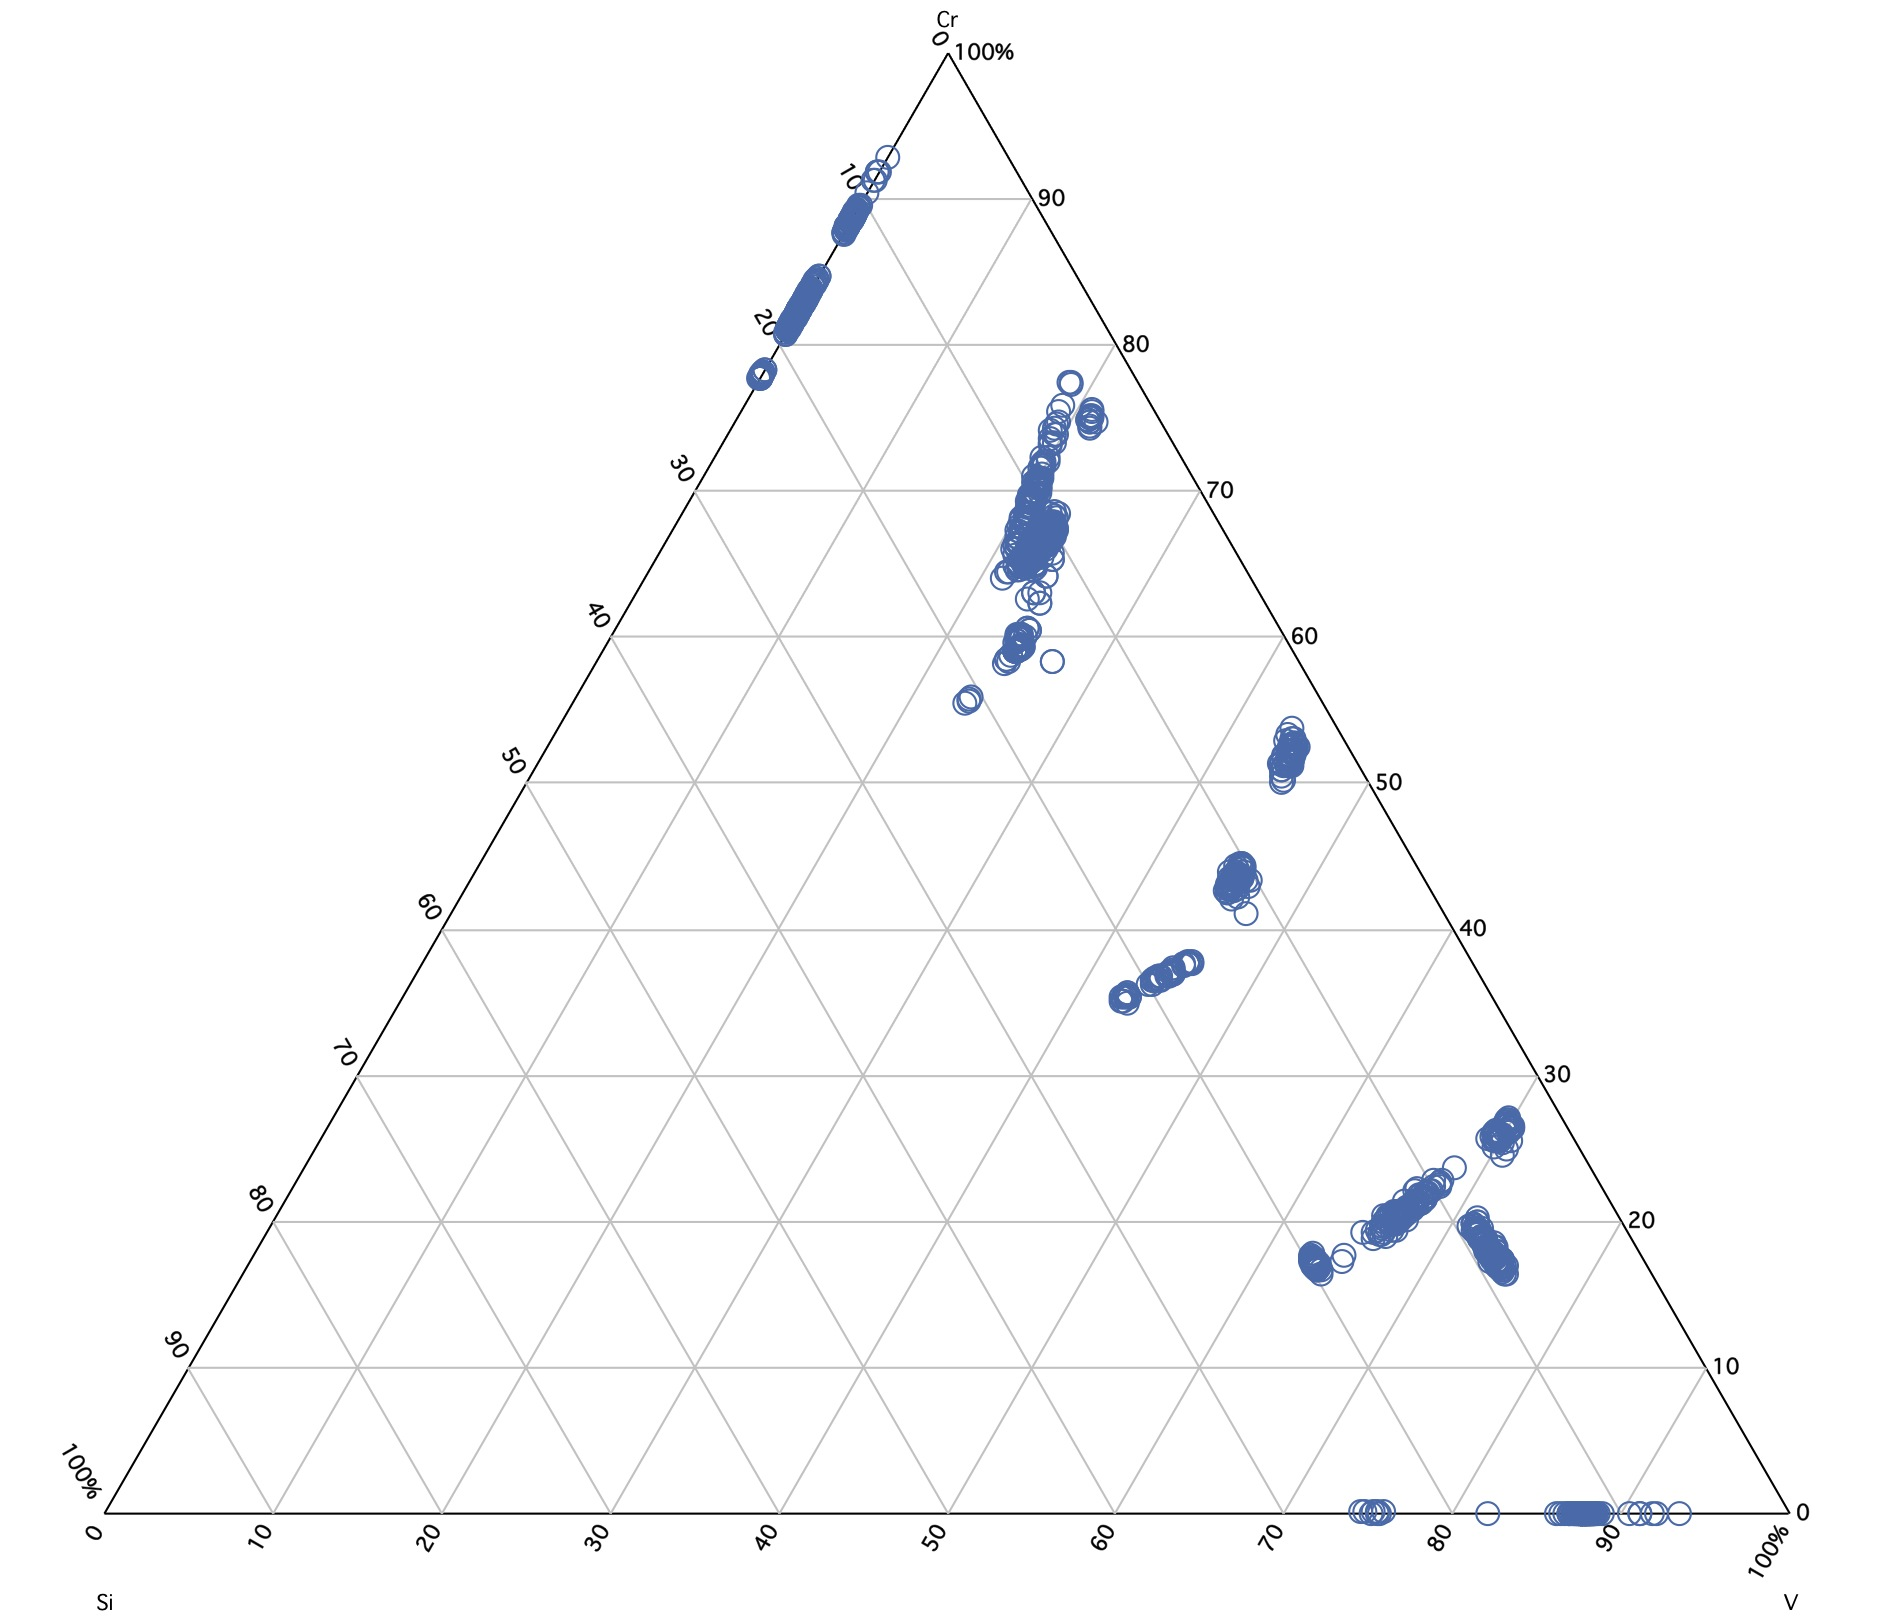
\includegraphics[width=16cm]{ternarymap}
\caption{ WDS-measured eutectic, solid-solution and X$_3$Si compositions collected for the five binary and ternary alloys plotted in a ternary map.}
\label{fig:ternarymap}
\end{figure}
%
%
\begin{landscape}\vspace*{\fill}
\begin{figure}[H]
\begin{center}
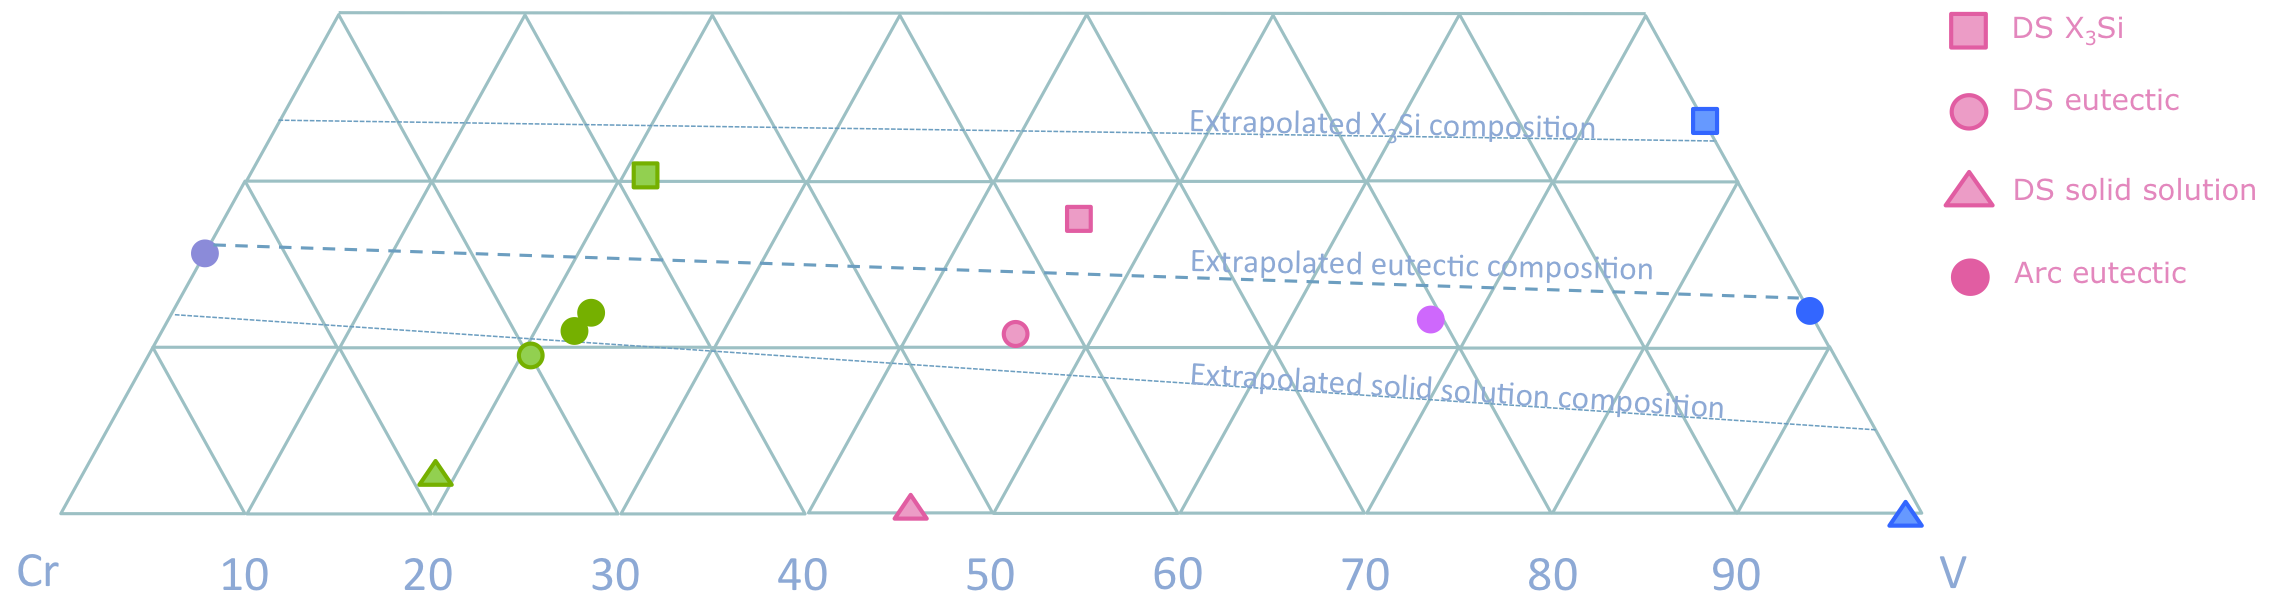
\includegraphics[width=24cm]{WDSaveragecompo}
\caption{Composition map of average bulk eutectic compositions and phase individual compositions of the five binary and ternary alloys.  Average bulk eutectic compositions were measured for non-directional-solidification manufacture ingots using a statistically random method.  Average individual phase compositions were measured in DS manufactured alloys only, as the lamellar spacing of arc-melt manufactured alloys were too small to provide sufficient analysis area for accurate measurements.}
\label{fig:WDSaveragecompo}
\end{center}
\end{figure}
\end{landscape}
%


Case 2.
The high viscosity of the melt means that a lamellar microstructure may grow into the melt with an equilibrium composition and equilibrium phase fraction, while rejecting unsuitable elements into the remaining melt.  The remaining melt then has to solidify with phase fractions that are atypical of eutectics at equilibrium.  The eutectic microstructure inherently has a large composition range.

Case 3. 
There were discrepancies in measured data due to the conditions in which composition measurements were performed.  The eutectics have a narrow composition range, but due to the interactions between the transition metals and silicon, accurate measurements cannot be made without bespoke intermediate WDS standards being used.  This issue has been raised by other scientists working on silicides. 

When determining potential peak overlaps using a simulation software package "virtual WDS",  the majority of overlapping peaks are found.  The output of this package is used to construct set-up file that detail the initial WDS acquisition conditions that would be evaluated for suitability, and reconfigured as required.  

Initially, WDS calibration was done with pure element standards at the start of the day.  Cr, Si and V were used for the binary and ternary alloys.  Measurements of the solid-solution phase would usually sum up to 100at.\%.  Measurements of the silicide phase were unreliable.  They consistently totalled to less than 100at.\%.  It was thought that interactions between Si and the transition metals in the alloys played a part in measurement inaccuracy. 
 
An intermediate standard, calcium fayalite, was then used.  This is a silicate containing calcium.  It was found that the measured total weight percent was less accurate than using element standards, and measured 96--98\%.  Repeated re-calibration with calcium fayalite showed that the WDS machine was consistently producing very accurate measurements of 100.0$\pm$0.3at.\% with different spot sizes and beam current intensities.  This suggests that an unknown interaction within the investigated silicide alloys is contributing to measurements consistently totalling less than 100\%.  An intermediate standard iron fayalite was tried.  Iron is a transition metal, and any interactions between transition metal and silicon would be accounted for when using iron fayalite as a standard.  Iron fayalite measurements fell within 100.0\% $\pm$0.15, but eutectic samples still produced results that consistently fell outside the 100.0\% $\pm$0.9 range.

Calibrations were slightly inconsistent for some elements.  For instance, the Ta  calibrations did not tally to 100wt.\% in the penultimate acquisition session, but were accurate in the last acquisition session.  There were no overlap with any peaks with the Ta M$_{\alpha}$ line.  A suitable explanation for the inconsistent measurements has not been found yet. 

Ideally, counters should be used in integral mode whenever possible to acquire data for the full range of an element's  peak; however, when there is substantial overlap of peaks, differential mode can be used to cut out some of the counts.  Differential mode was found to introduce additional error in the alloy system explored, and was not used. 
  
Exploration of the mineral collection at the Department of Earth Sciences at the University of Edi{n}urgh led to the conclusion that there are no known silicate minerals containing chromium, vanadium, tantalum or tungsten that could be used as a secondary standard.  Such a standard would need to be custom-made if more accurate measurements are required. 

The intermediate standard needs to have no grain boundaries visible.  Its composition has to be completely homogeneous.  Several manufacture options were explored.  The most sensible method was to purchase stock targets used for the physical vapour deposition (PVD) process.  These were made by plasma spraying.  The grain size of such samples is very small.  WDS is a method of measurement for a homogeneous, single-phase material.  Using a secondary standard with many grain boundaries would introduce additional measurement error that cannot be accurately quantified.  Significant expense and effort would be required to follow the idea through, with a good chance of no improvement in measurement accuracy.  This idea was not pursued further.  Instead, further tinkering about with different standards was done to increase accuracy.  Slightly unusual calibrations standards for Al and Si have been used in this project.  Due to the issues faced with collecting good data in this system, calibrations have been adapted to best suit the alloy systems.  Pure silicon works better than fayalite and wollastonite for Si calibration, but zirconium silicate was later found to produce better data, and was used for the last set of data acquired.  Orthoclase, a potassium aluminium silicate, was used for the latest period of Al calibrations.

Prior to acquiring a new set of data, the optical focus of sample needs to be optimised for accurate data acquisition.  BSE mode, the mode that is used for specimen exploration, is insensitive to suboptimum sample height and can appear focussed with the lack of optical focus.

Measured eutectic compositions of the binary and ternary alloys using grids of large spots have been plotted in Figure \ref{fig:ternarymap}.  All composition ranges are quite large, sitting along strict lines between their corresponding pair of solid-solution and intermetallic.  As the lamellae are not infinitesimally small compared to the analysis spot size, data scatter due to the analysis volumes having different volume fractions of intermetallic would be statistically significant.

The arc-melted and PM manufactured alloys that have high chromium content have a fine lamellar structure that does not allow for accurate spot analysis of individual phases.  These alloys need to be solidified more slowly to obtain the coarser lamellae required for spot analysis.
%

\section{Microstructure and WDS Analysis of Binary and Ternary Alloys}

\subsection{WDS Area Maps}

WDS area maps of the two binaries were collected, with the highest possible resolution that can be configured in the WDS machines, in the hope that elemental segregation within each eutectic cell could be detected.  Although the beam spot diameter was set to 0.1\micro\metre, the exact resolution depends on the interaction volume of the beam, which is typically 2\micro\metre.  Three detectors were set to collect information from the metal element: Cr or V.  Two detectors were set to collect information from Si.  Each map took 14 hours to complete.  In the DS Cr--Cr$_3$Si eutectic (Figure \ref{fig:creutmap}), interlamellar spacing was of the same size as the WDS spot size.  As a result, the map does not have sufficient resolution to look at partitioning in detail.  This alloy was manufactured with a very slow withdrawal rate of 20-40\milli\metre/hour; the small interlamellar spacing is an intrinsic property of Cr--Cr$_3$Si.  The peripheries of eutectic cells have different compositions in neighbouring grains.  The periphery intermetallic phase  is dark orange (high Si content) in the first quadrant and pale orange in the fourth quadrant of Figure \ref{fig:creutmap}b.  These neighbouring eutectic cells, despite having been very slowly cast using DS manufacture, have different phase compositions.  Further, the phase fractions are different at neighbouring periphery areas; the first quadrant has lower intermetallic phase fraction than the fourth quadrant.  Although the direction a specimen is sectioned relative to its orientation affects the phase fraction seen to some extent, we will demonstrate that variation in phase fraction, together with variation in phase compositions, are evidence that melt viscosities in these systems are very high, and melt mixing achieved is poor across all the manufacture methods explored.

In the semi-quantitative map for ($\frac{3}{4}$Cr, $\frac{1}{4}$V)--($\frac{3}{4}$Cr, $\frac{1}{4}$V)$_3$Si) (Figure \ref{fig:tereutmap}), the microstructure is coarse enough to resolve elemental segregation within individual phases.  There is a slight segregation of Cr in the cores of coarser solid-solution.  No segregation is seen within the  eutectic cells.  The lighter blue zone seen at the top of the Si map is probably due to acquisition error.

The DS V--V$_3$Si eutectic (Figure \ref{fig:veutmap}), with a 20mm/hour withdrawal rate during manufacture, had a microstructure that was barely coarse enough to obtain sufficiently good data.  Due to the microstructural coarseness, a composition map of only a part of a eutectic cell was made.  The Si content of the solid-solution within the eutectic cell appears black with a few pixels of dark blue (Figure \ref{fig:veutmap}b), indicating a lower content than at the cell periphery (dark blue interspersed with black).  The interfaces between the solid-solution and intermetallic phases appear pixelated in intermediate colours of yellow and green.  It would have been better statistically to accumulate good data for 2 eutectic cell neighbours to look at cellular elemental segregation, but data collection would have taken more than a day.  This was deemed an ineffective allocation of the WDS facility, and we decided against doing so.

%
\begin{landscape}
\begin{figure}
\begin{center}
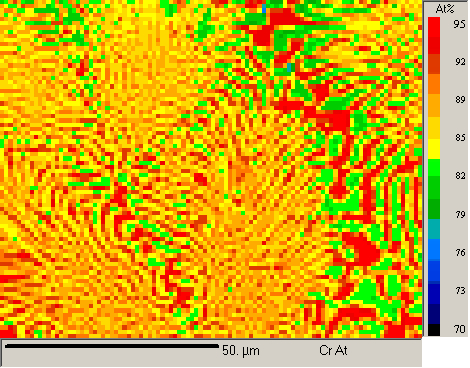
\includegraphics[width=11cm]{creutCrmap}
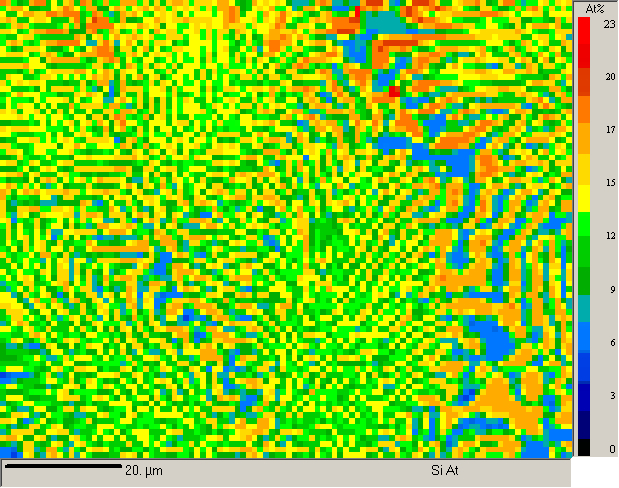
\includegraphics[width=11cm]{creutSimap}
\caption{WDS maps in at.\%\ of (a) Cr and (b) Si in DS Cr--Cr$_3$Si.}
\label{fig:creutmap}
\end{center}
\end{figure}
\end{landscape}
%

%
\begin{landscape}
\begin{figure}
\begin{center}
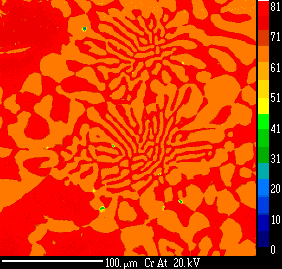
\includegraphics[width=7.2cm]{middle_Cr}
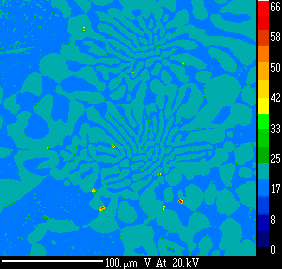
\includegraphics[width=7.2cm]{middle_V}
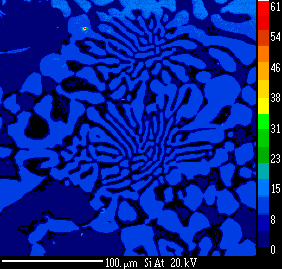
\includegraphics[width=7.2cm]{middle_Si}
\caption{WDS maps in at.\%\ of (a) Cr, (b) V and (c) Si in DS ($\frac{3}{4}$Cr, $\frac{1}{4}$V)--($\frac{3}{4}$Cr, $\frac{1}{4}$V)$_3$Si.}
\label{fig:tereutmap}
\end{center}
\end{figure}
\end{landscape}
%

%
\begin{landscape}
\begin{figure}
\begin{center}
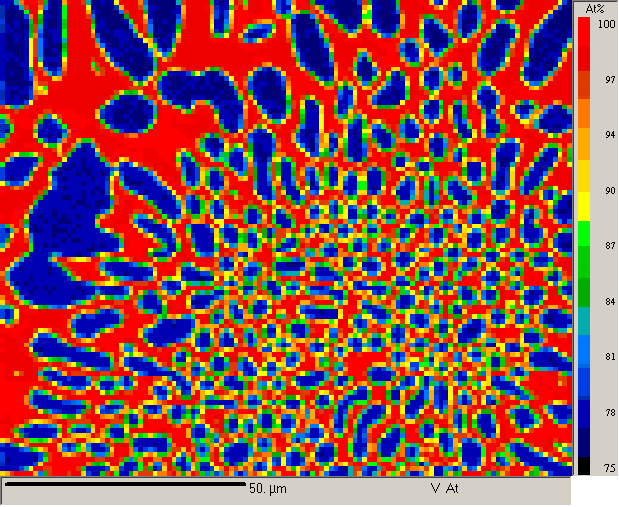
\includegraphics[width=11cm]{veutVmap}
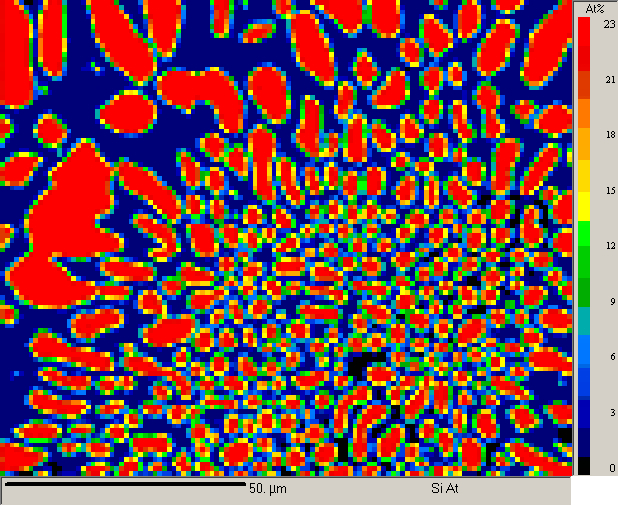
\includegraphics[width=11cm]{veutSimap}
\caption{WDS maps in at.\%\ of (a) V and (b) Si in DS V--V$_3$Si.  Although this microstructure is a lot coarser than the Cr--Cr$_3$Si eutectic, the resolution is insufficient to determine whether there is elemental segregation in the solid-solution at phase boundaries.}
\label{fig:veutmap}
\end{center}
\end{figure}
\end{landscape}
%
%
%\begin{landscape}\vspace*{\fill}
%\begin{figure}
%\begin{center}
%\includegraphics[width=24cm]{set}
%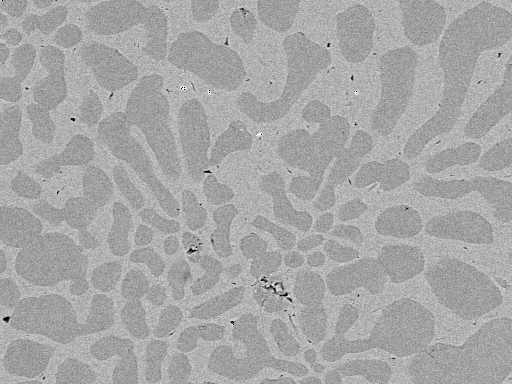
\includegraphics[width=4cm]{75VRF}
%\caption{Micrographs of the Binary and Ternary Alloys.  The alloys in first row are micrographs of non-DS manufactured.  The second and third rows are micrographs of transverse and longitudinal views of DS manufactured alloys.}
%\label{fig:set}
%\end{center}
%\end{figure}
%\end{landscape}
%


\subsection{Binary Alloy Cr--Cr$_3$Si}

\subsubsection{Non-Directional Solidification Manufactured Ingots}
The Cr--Cr$_3$Si alloy has a lamellar microstructure with the smallest interlamellar spacing out of all the alloys studied (Figure \ref{fig:Crarctrans}).  It was very difficult to manufacture an ingot with lamellar structure as the majority structure due to a combination of factors.  All manufacture routes employed in this work did not have means to provide adequate melt mixing.  The very high melt viscosity, exacerbated by the high chromium and silicon contents of this composition, resulted in a melt with localised inhomogenieties that were conducive for the nucleation and growth of dendrites ahead of the solidification front. 

The large difference between the melting points of chromium and silicon also causes chromium to experience substantial volatilisation during manufacture when ingot feedstock is in elemental form.  This is especially the case when elemental feedstock experiences very high temperatures.  Arc-melted, PM manufactured and horizontal RF manufactured specimens all fall within these boundaries.  Many iterations of composition adjustments had to be performed to achieve a microstructure that was not dominated by dendrites on a macro-scale as seen in the arc-melt manufactured specimen in Figure \ref{fig:Crarctrans}.

 %
\begin{figure}[H]
\begin{center}
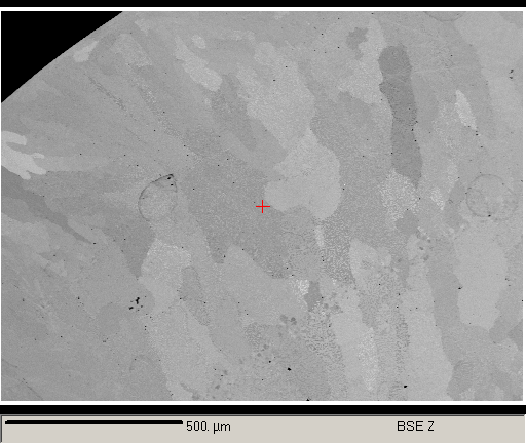
\includegraphics[width=10cm]{Cr_arc_trans}
\caption{Transverse section of an arc-melt manufactured Cr--Cr$_3$Si ingot showing many grains of eutectic microstructure of different orientation.}
\label{fig:Crarctrans}
\end{center}
\end{figure}
%
 
This composition, when non-dendritic, had quite an orderly lamellar microstructure (Figures \ref{fig:Crarctrans} and \ref{fig:Crarcsample1}).  A less orderly lamellar microstructure could be seen in some areas (Figure \ref{fig:Crarcsample1c}).  These non-directional ingots were suitable for grid analysis for bulk composition measurements, but the interlamellar spacing was too small to allow for accurate analysis of the individual phases, despite using the smallest possible WDS beam configuration for analysis.  There was substantial interference from the opposite phase, which resulted in inaccurate data collected.  The less orderly lamellar microstructure was also too fine for individual phase analysis.

%

\begin{figure}[H]
\begin{center}
%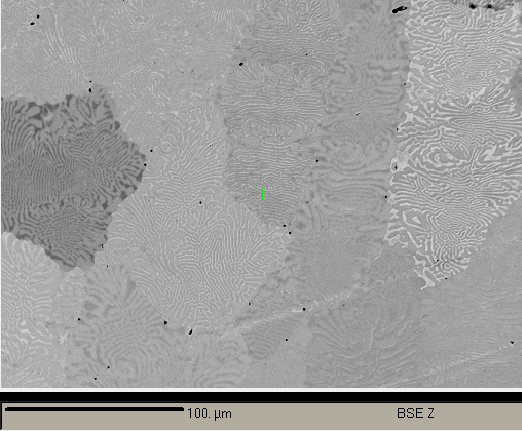
\includegraphics[width=10cm]{_Jun18sample1_circle_middle_50um_bse_scale}
%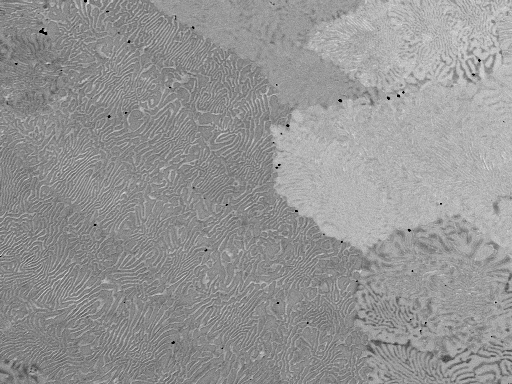
\includegraphics[width=8cm]{_Jun18_sample_1_circle_sidei_50um}
%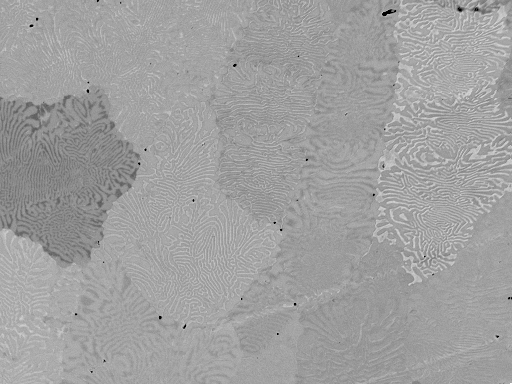
\includegraphics[width=8cm]{_Jun18sample1_circle_middle_50um_bse}
%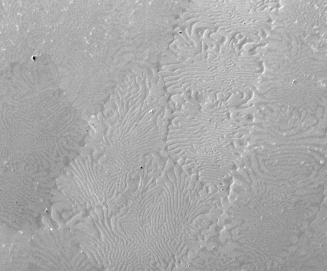
\includegraphics[width=10.5cm]{_Jun18_sample_1_circle_side_50um_SE_middle}
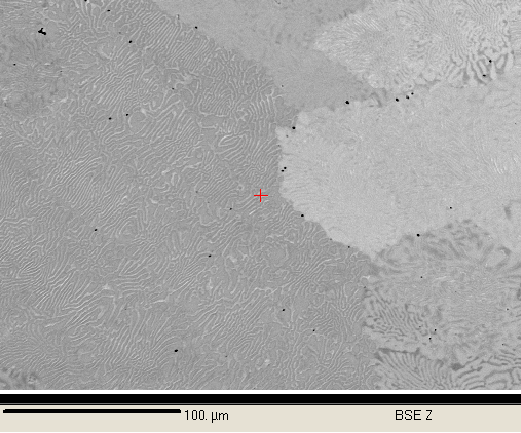
\includegraphics[width=8cm]{_Jun18_sample_1_circle_sidei_50um_scale}
\caption{BSE micrograph of typical eutectic microstructure in compensated arc-melt manufactured Cr--Cr$_3$Si (-1.05wt.\% Si.)}
\label{fig:Crarcsample1}
\end{center}
\end{figure}
%
%
%\begin{figure}[H]
%\begin{center}
%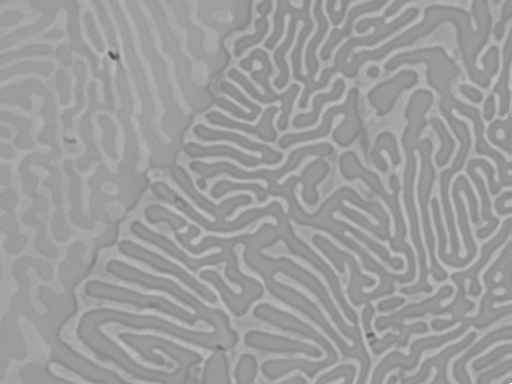
\includegraphics[width=10cm]{_Jun18_sample_1_circle_middle_10um_bse_ii_points}
%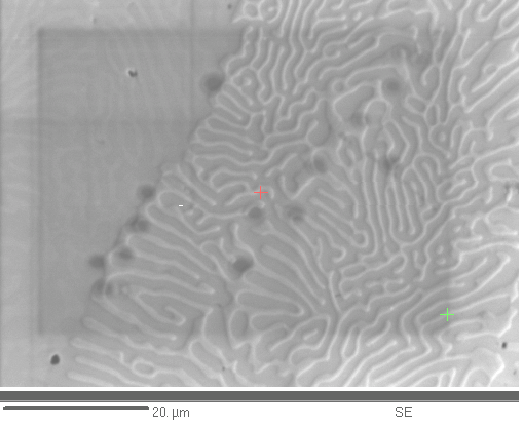
\includegraphics[width=10.5cm]{_Jun18_sample_1_circle_middle_10um_bse_ii_points_afterSE}
%\caption{As seen from the burn marks from the beam after analysis, the microstructure was found to be too fine to allow for accurate analysis of either phase without interference from each other.  This was confirmed by WDS data.}
%\label{fig:Crarcsample1zoom}
%\end{center}
%\end{figure}
%
%

\vspace*{\fill}
\begin{figure}[H]
\begin{center}
%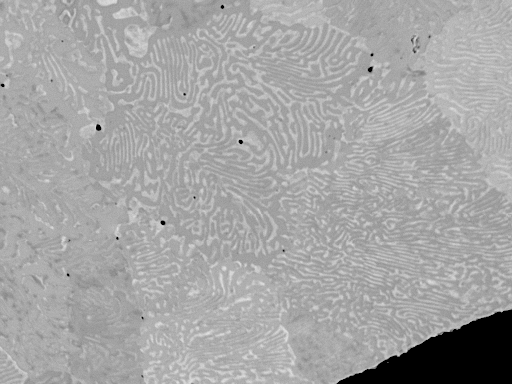
\includegraphics[width=7.2cm]{_Jun18_sample_1_circle_sideii_50um}
%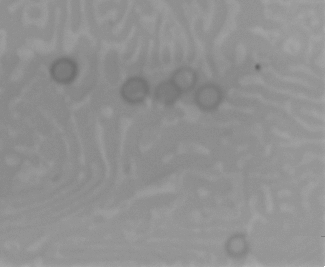
\includegraphics[width=7.2cm]{_Jun18_sample_1_circle_sideii_10um}
%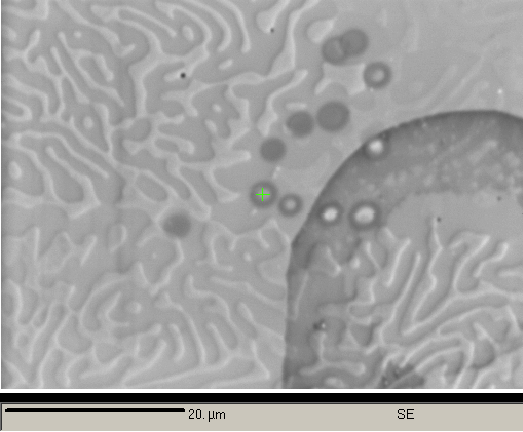
\includegraphics[width=10cm]{_Jun18_09_Jun18_Morning_sample_1_circle_sideiv_10um_scale}
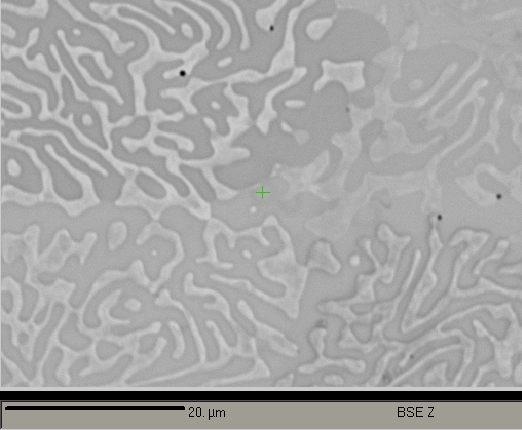
\includegraphics[width=8cm]{_Jun18_sample_1_circle_sideiv_10um_bse_scale}
%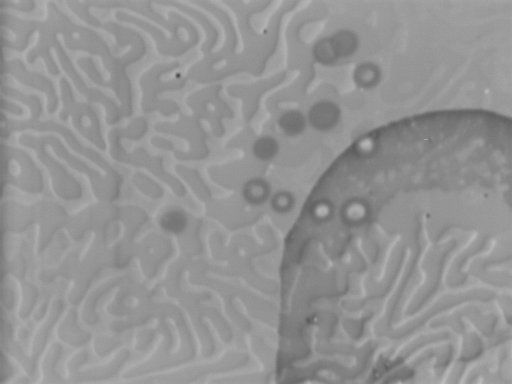
\includegraphics[width=7.2cm]{_Jun18_sample_1_circle_sideiv_10um}
%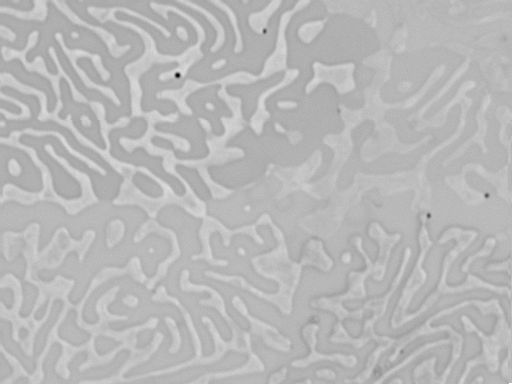
\includegraphics[width=7.2cm]{_Jun18_sample_1_circle_sideiv_10um_bse}
%\includegraphics[width=7.2cm]{_Jun18_09_Jun18_Morning_sample_1_circle_sideii_20um_scale}
%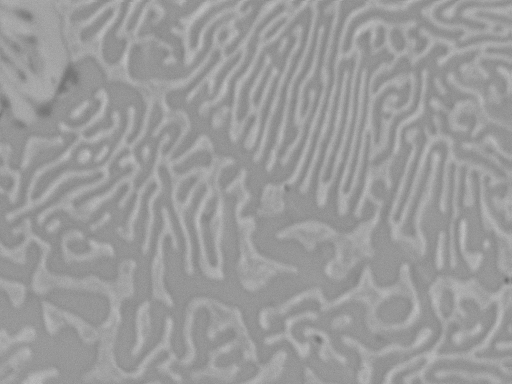
\includegraphics[width=7.2cm]{_Jun18_sample_1_circle_side_v_10um_bse_before}
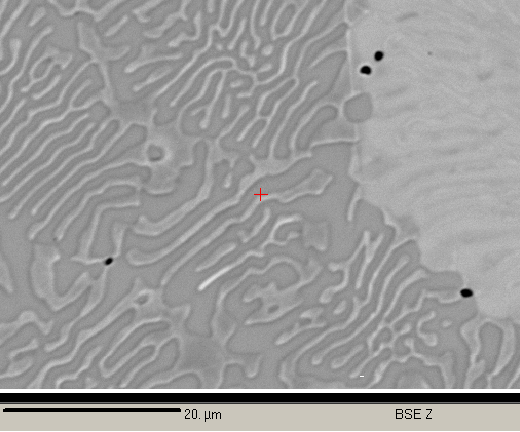
\includegraphics[width=7.95cm]{_Jun18_sample_1_circle_sidei_20um_scale}
\caption{BSE micrographs of another location of typical eutectic microstructure in compensated arc-melt manufactured Cr--Cr$_3$Si.}
\label{fig:Crarcsample1c}
\end{center}
\end{figure}
%\end{landscape}
%

\subsubsection{Directional Solidification Manufactured Ingots}

In ingots manufactured by very slow DS manufacture using a RF furnace or a mirror-image furnace, inadequate melt mixing resulted in dendritic structures nucleating and solidifying ahead of the intentionally very slow solidification front.  In fact, the slowness probably allows the dendrites that have formed to remain very much ahead.  The left-over melt composition, being substantially further away from eutectic composition, together with the break-down of the planar solidification front, cause non-lamellar structures to form from the rest of the melt (Figure \ref{fig:Cr100middle20umeutectic}).

In one instance, when a suitable non-dendritic composition developed in a planar front near the beginning of a cast, the lamellar microstructure failed to form (Figure \ref{fig:location171crrfpointsSS}).  This is very curious.  Perhaps the composition was too far away from eutectic composition to allow lamellae to form.  Point analysis of the individual phases were performed.   Analyses locations have been marked (Figure \ref{fig:location171crrfpointsSS}).  Individual phase analysis is not possible on arc-melt manufactured specimens due to the smal interlamellar spacing.  Solid-solution measurements were consistently high, between 100.5\% and 101.2\%.  Silicide total weight measurements for this location ranged between 101.1\% and 101.9\%, with a Si content of 13.1-13.6 wt.\%.  The narrow composition ranges show that WDS measurements are consistent, even though they are higher than the accepted maximum value of 100.8\%.

%
\begin{figure}[H]
\begin{center}
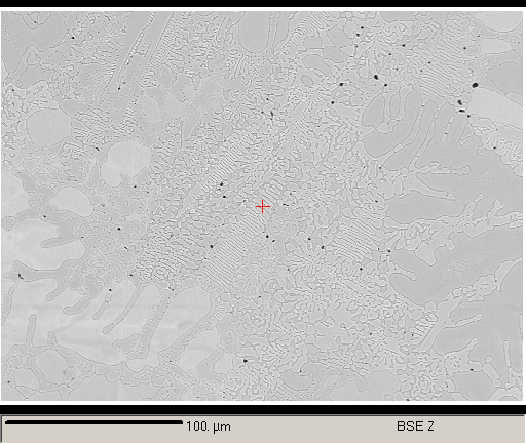
\includegraphics[width=10cm]{Cr100middle20umeutectic}
\caption{A small region of eutectic microstructure in a Cr--Cr$_3$Si.  Dendrites of both phases flank it,  with the solid-solution (lighter dendrite) on the left, and intermetallic (darker dendrite) on the right, which makes it difficult to establish a regular microstructure due to solidification-front perturbation.}
\label{fig:Cr100middle20umeutectic}
\end{center}
\end{figure}
%
%
\begin{figure}[H]
\begin{center}
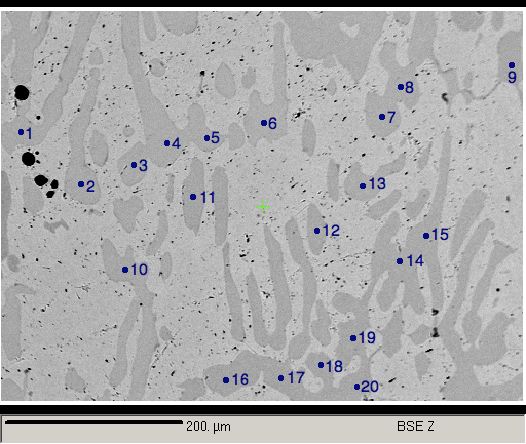
\includegraphics[width=12.5cm]{location171crrfX3Sipoints} 
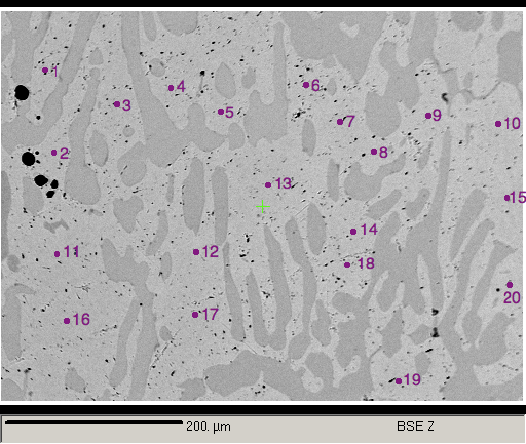
\includegraphics[width=12.5cm]{location171crrfpointsSS}
\caption{(a) Solid-solution and (b) X$_3$Si analyses in DS manufactured Cr--Cr$_3$Si, with an analysis spot diameter of 1\micro\metre.}
\label{fig:location171crrfpointsSS}
\end{center}
\end{figure}
%\end{landscape}
%
\subsection{Ternary Alloy ($\frac{3}{4}$Cr, $\frac{1}{4}$V)--($\frac{3}{4}$Cr, $\frac{1}{4}$V)$_3$Si}

Microstructures of this composition were quite orderly, and interlamellar spacing remained small when manufactured by methods with large undercooling (Figures \ref{fig:Cr75less3Sigii} and \ref{fig:75CrlongiBSE}).  Melt viscosity was similar to the Cr--Cr$_3$Si binary based on visual examination during arc-melting and horizontal RF manufacture. 


\subsubsection{Non-Directional Solidification Manufactured Ingots}
Only arc-melt manufactured ingots were produced.  This composition was not PM manufactured due to extensive facility accessibility difficulties and long turn-around time for manufacture.  Elemental segregation can be seen in the first quadrant of Figure \ref{fig:75CrlongiBSE}.  BSE micrographs after area analysis using a grid of 15\micro\metre\ spots show contamination  caused by analysis (Figure \ref{fig:75CrgridiiSEafter}).  These spots do not overlap, and the acquired data is sound.  Data acquired from grids that had overlap were discarded (Figure \ref{fig:75CrgridiiiSEafter}).  Alloy microstructural detail can be observed  (Figures \ref{fig:75CrgridiiSEafter}b and \ref{fig:75CrgridiiiSEafter}b).  The spot size is large enough to accurately determine bulk composition when large grids of spots are taken.

%
\begin{figure}[H]
\begin{center}
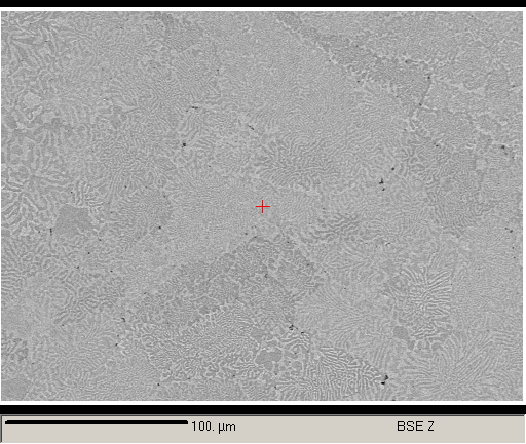
\includegraphics[width=11cm]{Cr75less3Sigii}
%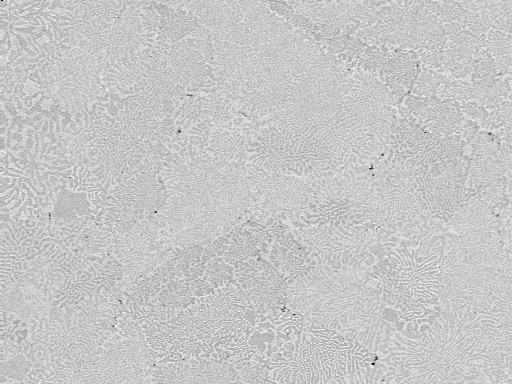
\includegraphics[width=11cm]{_Sep6_75Cr_gridii_beforeBSE}
\caption{Location for a grid of 25\micro\metre\ diameter spot analysed in the eutectic microstructure of arc-melt manufactured ($\frac{3}{4}$Cr, $\frac{1}{4}$V)--($\frac{3}{4}$Cr, $\frac{1}{4}$V)$_3$Si (-3 at.\% less Si).}
\label{fig:Cr75less3Sigii}
\end{center}
\end{figure}
%
%
\begin{figure}[H]
\begin{center}
%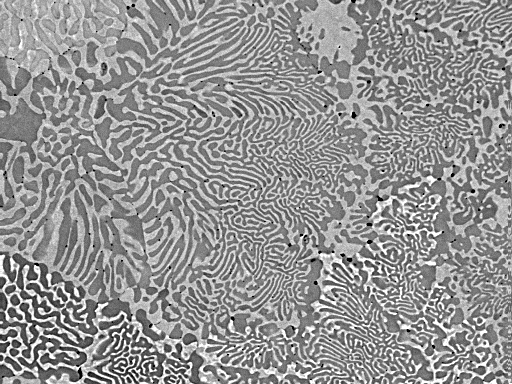
\includegraphics[width=11cm]{_Sep6_75Cr_aug09}
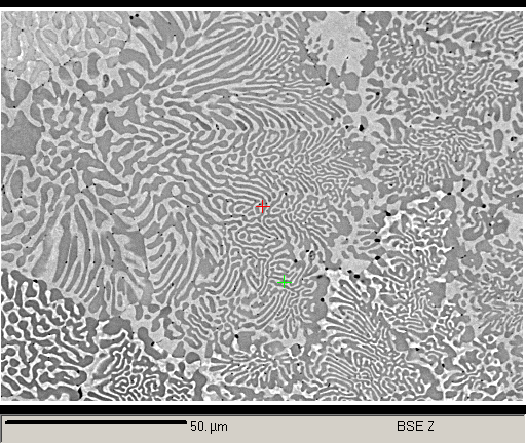
\includegraphics[width=11cm]{_Sep6_75Cr_eut_scale_aug09.png}
\caption{(a) Longitudinal cross section of the eutectic microstructure of arc-melt manufactured ($\frac{3}{4}$Cr, $\frac{1}{4}$V)--($\frac{3}{4}$Cr, $\frac{1}{4}$V)$_3$Si (-3 at.\%\ less Si.)}
\label{fig:75CrlongiBSE}
\end{center}
\end{figure}
%
%
\begin{figure}[H]
\begin{center}
%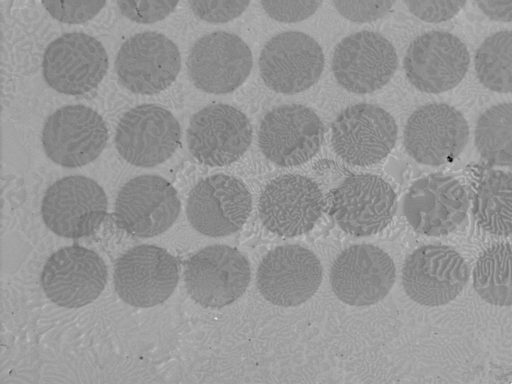
\includegraphics[width=8cm]{_Sep6_75Cr_eut_3Si_transv_K_30_grid_ii_after_BSE_3rd_quadrant}
%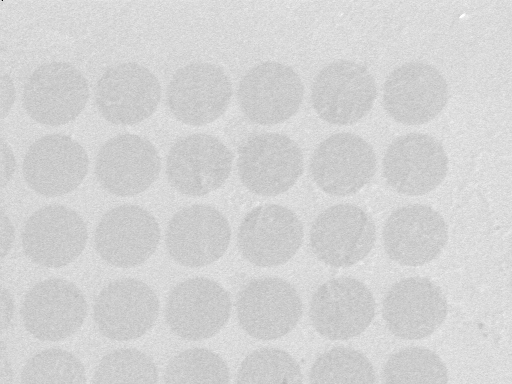
\includegraphics[width=8cm]{_Sep6_75Cr_eut_3Si_grid_ii_after_BSE_2nd_quadrant}
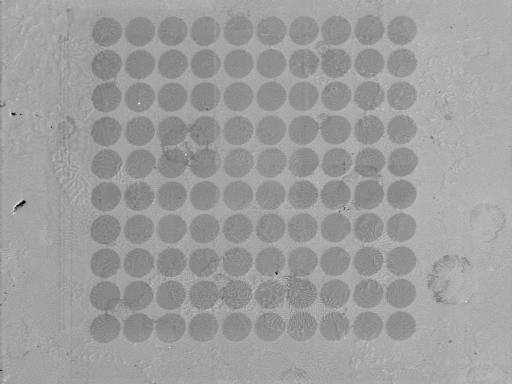
\includegraphics[width=7.8cm]{_Sep6_75Cr_eut_3Si_grid_ii_after_SE_full_grid}
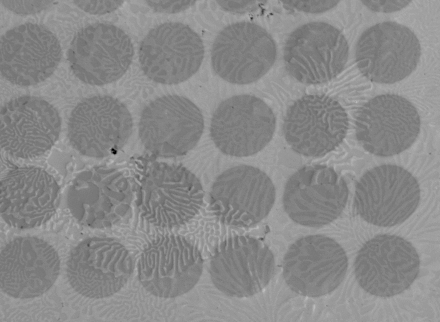
\includegraphics[width=8cm]{_Sep6_75Cr_eut_3Si_grid_ii_after_BSE_4th_quadrant}
\caption{ (a) BSE micrograph of contamination marks left by a grid of 25\micro\metre\ diameter spots analysed in the eutectic microstructure of arc-melt manufactured ($\frac{3}{4}$Cr, $\frac{1}{4}$V)--($\frac{3}{4}$Cr, $\frac{1}{4}$V)$_3$Si (-3 at.\%\ less Si), (b) close-up of the grid's fourth quadrant to illustrate that the large spot size relative interlamellar spacing allowed for good statistics of the bulk composition to be collected.)}
\label{fig:75CrgridiiSEafter}
\end{center}
\end{figure}
%
%
\begin{figure}[H]
\begin{center}
%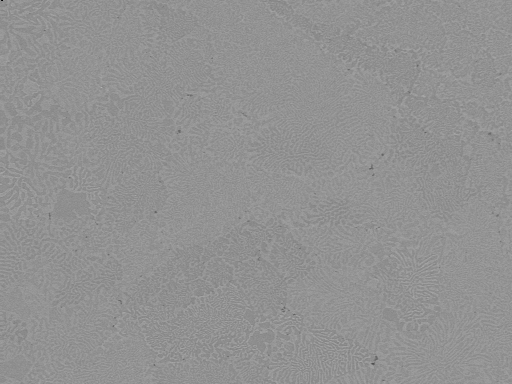
\includegraphics[width=8cm]{_Sep6_75Cr_3Si_transv_K_30_grid_ii_before_BSE}
%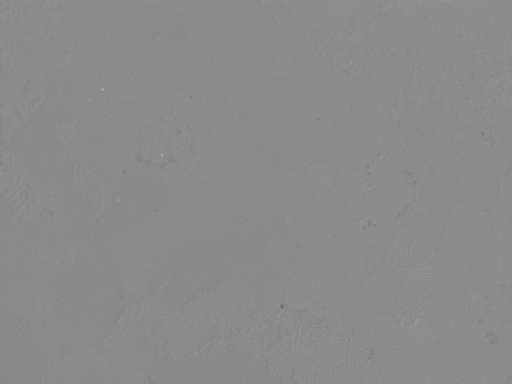
\includegraphics[width=8cm]{_Sep6_75Cr_eut_3Si_transv_K_30_grid_ii_before_SE}
%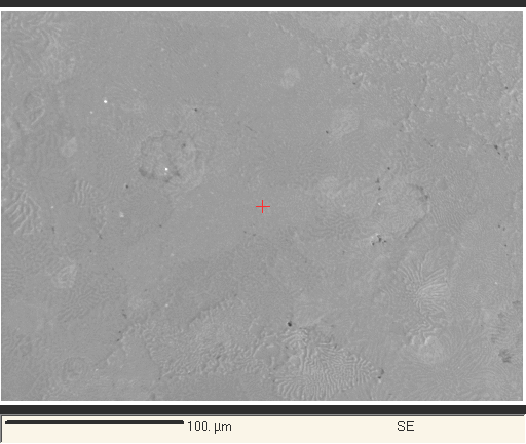
\includegraphics[width=8cm]{_Sep6_75Cr_eut_3Si_transv_K_30_grid_ii_scale_scale}
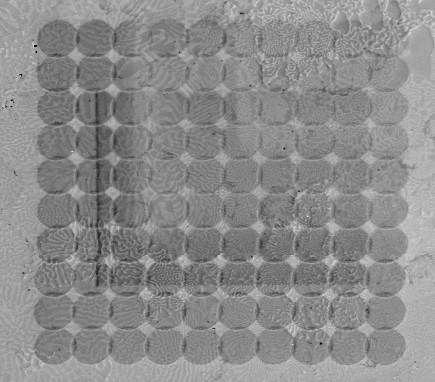
\includegraphics[width=7.7cm]{_Sep6_75CrafterSE}
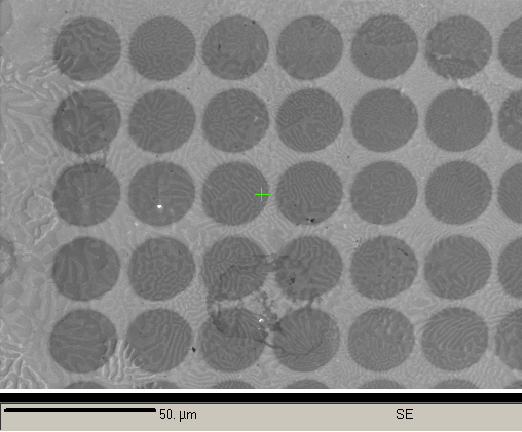
\includegraphics[width=8.2cm]{Sep675Cr_eut_minus3Si_gridii_scaleafterBSE}
\caption{Micrographs in BSE showing contamination marks of a grid of 25\micro\metre\ diameter spots analysed by WDS in the eutectic microstructure of DS ($\frac{3}{4}$Cr, $\frac{1}{4}$V)--($\frac{3}{4}$Cr, $\frac{1}{4}$V)$_3$Si (with -3 at.\%\ less Si): (a) first grid, with inadequate spacing between spots (b) close-up view of the second grid, with larger inter-spot spacing.)}
\label{fig:75CrgridiiiSEafter}
\end{center}
\end{figure}


 
%
\subsubsection{Directional Solidification Manufactured Ingots}
These ingots were analysed for individual phase analysis as their interlamellar spacing was a lot larger than the arc-melt manufactured ingots, which allowed for individual phase analysis without data from the other phase interfering with the results collected.

The obvious bright particles in Figure \ref{fig:75CrgridiiiBSE}, which are bright because of atomic number contrast, show that segregation of the heavier elements, occurring during solidification is not removed by the long time spent near the melting point during directional solidification.  Accurate diffusion data, which could be used to calculate the time required to homogenise the alloy does not exist, but if reasonable values are assumed, the mean free path at these temperatures can be calculated.  Thus if D$_0$ is assumed to be 5 x 10$^{-3}$ \square\metre/s and the activation energy for diffusion is assumed to be 5eV, then the mean free path, if the sample is assumed to be held at 1700\celsius\ (i.e. just below the melting point) for 1000s is found to be only about 1 \micro\metre.  Clearly, much longer times at temperature would be required to remove the segregation.

A more degenerate microstructure was also seen within the same ingot (Figure \ref{fig:75CrgridivBSE}).  Each eutectic cell is smaller, and there is a higher degree of coalescence.  There are more cells per unit area.  The middle of each eutectic cell is more globular, with very little lamellar structure.  This appeared near the ingot tip where solidification was first initiated.  This probably stems from the relatively slower rate of solidification experienced by the region.  It could also be that the region's composition has higher vanadium content than at the middle of the ingot.  It is not probable that the less lamellar structure is due to a sectioning effect. 

During the first few iterations of ingot manufacture, the compositions did not form such lamellar structures.  Aside from dendritic structures dominating ingots, there was one ingot that formed a degenerate eutectic structure with a high volume fraction of coarse solid-solution globules (Figure \ref{fig:75CrgridivBSE}b).  It was not feasible to determine the bulk composition using WDS large spot grid analysis due to microstructure coarseness.  Bulk composition measurements would be substantially affected by solid-solution volume fraction.  Phase analysis showed that the phases have very similar compositions to the alloys that have lamellae.

%
\begin{figure}[H]
\begin{center}
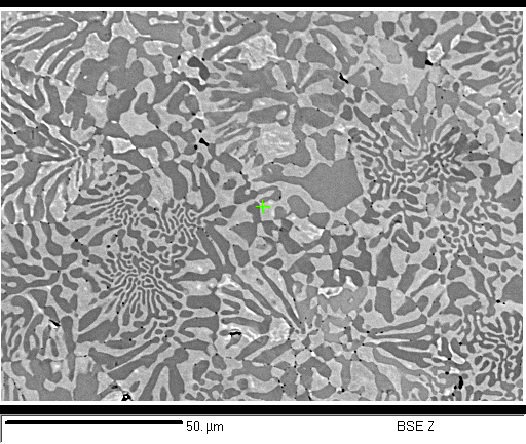
\includegraphics[width=7.92cm]{_Sep6_gridiii_75Cr_scale_beforeBSE}
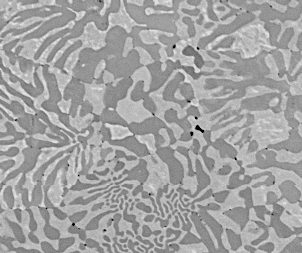
\includegraphics[width=8cm]{_Sep6_gridiii_75Cr_30BSE}
\caption{(a) A BSE micrograph of a good site for a grid of 25\micro\metre\ diameter large spot analyses to be conducted by WDS in the eutectic microstructure of DS ($\frac{3}{4}$Cr, $\frac{1}{4}$V)--($\frac{3}{4}$Cr, $\frac{1}{4}$V)$_3$Si.  This ingot has been compensated with 3at.\%\ less Si. (b) A magnified view of the top left corner.  Notice the segregation of elements present in the solid-solution that appears as paler spots.}
\label{fig:75CrgridiiiBSE}
\end{center}
\end{figure}

%

%
\begin{figure}[H]
\begin{center}
%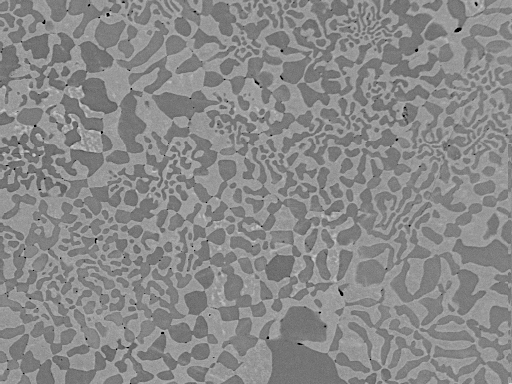
\includegraphics[width=11cm]{_Sep6_grid_iv_75Cr_beforeBSE}
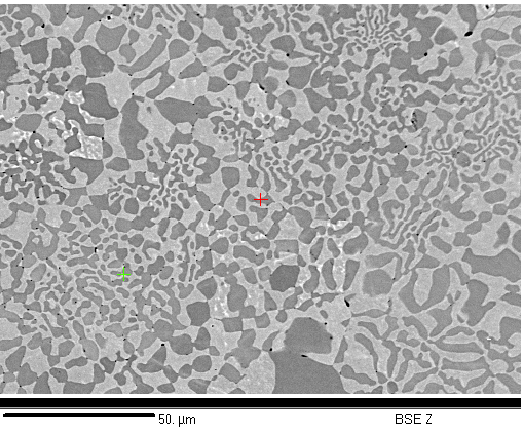
\includegraphics[width=8cm]{_Sep6_grid_iv_75Cr_scale_beforeBSE}
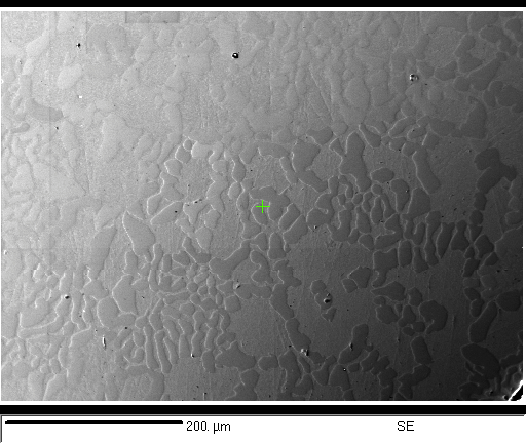
\includegraphics[width=7.9cm]{_Jun20_0975Cr25V_eut_comp_bham_arc_side_100um_BSE_scale}
\caption{(a) A BSE micrograph of a site with a more globular, less lamellar eutectic microstructure in DS ($\frac{3}{4}$Cr, $\frac{1}{4}$V)--($\frac{3}{4}$Cr, $\frac{1}{4}$V)$_3$Si (-3 at.\%\ less Si). (b) A microstructure of the same alloy that has some lamellar regions, and a large volume fraction of solid-solution.}
\label{fig:75CrgridivBSE}
\end{center}
\end{figure}
%


\subsection{Ternary Base Alloy \ilovewill{山}: ($\frac{1}{2}$Cr, $\frac{1}{2}$V)--($\frac{1}{2}$Cr, $\frac{1}{2}$V)$_3$Si}

($\frac{1}{2}$Cr, $\frac{1}{2}$V)--($\frac{1}{2}$Cr, $\frac{1}{2}$V)$_3$Si has been designated as the project's base alloy.  This eutectic grows along less specific planes than Cr--Cr$_3$Si, and it was easier to achieve a lamellar microstructure in this ternary than the binary Cr--Cr$_3$Si eutectic.  Perhaps there is a larger composition and undercooling window for the the lamellar structure to form.

The ingots manufactured by the DS process used arc-melted ingots as feed-stock.  The microstructure is on the verge of being too fine to allow for WDS phase analysis; locations had to be manually done one at a time to minimise error due to xy table movement that would occur in semi-automatic data acquisitions.  Points that fall between solid-solution and intermetallic values were discarded, as they do not accurately represent individual phase compositions.    


%
%\begin{figure}[H]
%\begin{center}
%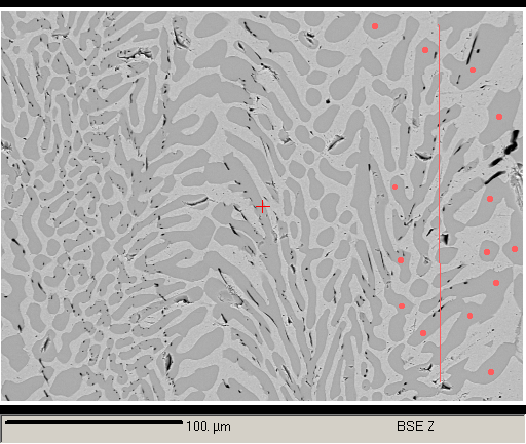
\includegraphics[width=10cm]{g05cirightsidex3si}
%\caption{A set of X$_3$Si WDS analyses of ($\frac{1}{2}$Cr, $\frac{1}{2}$V)--($\frac{1}{2}$Cr, $\frac{1}{2}$V)$_3$Si collected in within and on the perimeter of the right eutectic cell, with an analysis spot diameter of 1\micro\metre.}
%\label{fig:grid05cirightsidebeforeBSEx3si}
%\end{center}
%\end{figure}
%
%
%\begin{figure}[H]
%\begin{center}
%\includegraphics[width=10cm]{g05aSS}
%\caption{A set of solid-solution WDS analyses of ($\frac{1}{2}$Cr, $\frac{1}{2}$V)--($\frac{1}{2}$Cr, $\frac{1}{2}$V)$_3$Si collected in a eutectic cell, analysis spot diameter of 1\micro\metre.}
%\label{fig:g05aSS}
%\end{center}
%\end{figure}
%
%
%\begin{figure}[H]
%\begin{center}
%\includegraphics[width=10cm]{g05aX3Si}
%\caption{A set of solid-solution WDS analyses of ($\frac{1}{2}$Cr, $\frac{1}{2}$V)--($\frac{1}{2}$Cr, $\frac{1}{2}$V)$_3$Si collected in the periphery of a eutectic cell, analysis spot diameter of 1\micro\metre.  The line across the micrograph merely serves as a reference for the order that the analyses were taken.}
%\label{fig:g05aX3Si}
%\end{center}
%\end{figure}
%
%
\begin{figure}[H]
\begin{center}
\includegraphics[width=10cm]{g05bSS}
\caption{A set of solid-solution WDS analyses of ($\frac{1}{2}$Cr, $\frac{1}{2}$V)--($\frac{1}{2}$Cr, $\frac{1}{2}$V)$_3$Si collected in the periphery of a eutectic cell, analysis spot diameter of 1\micro\metre, designated as location b.  The line across the micrograph merely serves as a reference for the order that the analyses were taken.}
\label{fig:g05bSS}
\end{center}
\end{figure}
%
%
\begin{figure}[H]
\begin{center}
\includegraphics[width=10cm]{g05bX3Si}
\caption{A set of X$_3$Si WDS analyses of ($\frac{1}{2}$Cr, $\frac{1}{2}$V)--($\frac{1}{2}$Cr, $\frac{1}{2}$V)$_3$Si collected in the periphery of a eutectic cell, analysis spot diameter of 1\micro\metre, in location b.  The line across the micrograph merely serves as a reference for the order that the analyses were taken.}
\label{fig:g05bX3Si}
\end{center}
\end{figure}
%

%
%\begin{figure}[H]
%\begin{center}
%\includegraphics[width=10cm]{cr50bigspotsii100um}
%\caption{Locations of X$_3$Si compositions in arc-melt manufactured ($\frac{1}{2}$Cr, $\frac{1}{2}$V)--($\frac{1}{2}$Cr, $\frac{1}{2}$V)$_3$Si of WDS large spot analysis, with variable spot diameter of 10 or 15\micro\metre. }
%\label{fig:cr50bigspotsii100um}
%\end{center}
%\end{figure}
%
%
%\begin{figure}[H]
%\begin{center}
%\includegraphics[width=10cm]{g05abcSEafter}
%\caption{Contamination spots of WDS analyses of individual phases of DS manufactured ($\frac{1}{2}$Cr, $\frac{1}{2}$V)--($\frac{1}{2}$Cr, $\frac{1}{2}$V)$_3$Si, showing whether xy-table drift occurred between pin-pointing a spot for analysis and analysis completion.  The beam has a circular cross-section, with the analysis volume in the middle of its corresponding contamination spot.}
%\label{fig:g05abcSEafter}
%\end{center}
%\end{figure}
%
%

\begin{table}[htdp]
\begin{center}
\begin{tabular}{lcccccccc}
\hline
Alloy 			& Phase &Location/Analysis Type		&   Cr    		&  V 		      & Si   	\\
\hline
\hline
			
\ilovewill{山}	&	X$_3$Si pts&	bi						&37.05			&44.86			&18.08\\
				&	X$_3$Si pts&	bii					&37.20			&44.87			&17.93\\
				&	X$_3$Si pts&	c eutectic cell middle	&36.69			&44.19			&19.13\\

				& solid-solution&	b 					&52.79			&44.27			&2.95\\
				&solid-solution &ci eutectic cell middle		&51.67			&44.53			&3.79\\
				&solid-solution& ci eutectic cell periphery	&51.19			&44.28			&4.53\\

				&bulk composition	&grid of 10 by 10		&43.31			&45.51			&11.18\\
%	for1/4Cr	&bulk composition	&grid of 10 by 10			&20.79			&66.86			&12.34\\ 
%				& bulk composition	&grid of 10 by 10		&18.16			&73.11			&8.74\\			
%bulk arc g05 25um	
%b should be split into bi and bii	
%bulk arc melt g06 07
\hline
\end{tabular}
\end{center}
\caption{Average phase and bulk compositions of spot analyses at various locations in \ilovewill{山}.  All values are within 100 $\pm$ 0.8wt.\%.}
\label{tab:sanpoints}
\end{table}


For the solid-solution in area b (Figure \ref{fig:g05bSS}), there were a few analysis points that totalled above 100.8wt.\%.
These points had higher Si contents than the majority of points.  Good data was acquired at locations bi and bii (Figure \ref{fig:g05bX3Si}).  No points needed to be excluded.  The reason for the acquisition of good data was not found.  The composition of X$_3$Si within the eutectic cell and at the periphery of the eutectic cell were essentially identical for location b.  There was a very slight difference in composition between locations b (Figure \ref{fig:g05bSS}) and c (Figure \ref{fig:g05c}).   It had a Si content that was 1at.\% higher than locations bi and bii (Figure \ref{fig:g05bX3Si}).  Good data was also acquired; only a few points were excluded.  The bulk composition was measured at several locations, but only the average for one grid of 10x10 large spots have been presented in Table \ref{tab:sanpoints}.  Almost all measurements in this dataset fell within 100.0$\pm$0.8wt.\%.

%
\begin{figure}[H]
\begin{center}
\includegraphics[width=10cm]{g05cSS}
\includegraphics[width=10cm]{g05cpointsx3si}
\caption{A set of solid-solution and X$_3$Si WDS phase analysis locations of ($\frac{1}{2}$Cr, $\frac{1}{2}$V)--($\frac{1}{2}$Cr, $\frac{1}{2}$V)$_3$Si collected in a eutectic cell, analysis spot diameter of 1\micro\metre, designated as location c.}
\label{fig:g05c}
\end{center}
\end{figure}
%
\subsection{Ternary Alloy ($\frac{1}{4}$Cr, $\frac{3}{4}$V)--($\frac{1}{4}$Cr, $\frac{3}{4}$V)$_3$Si}

The ($\frac{1}{4}$Cr, $\frac{3}{4}$V)--($\frac{1}{4}$Cr, $\frac{3}{4}$V)$_3$Si eutectic has a distinctly non-facetted non-linear solidification front (Figures \ref{fig:grid08neighbouriSS}, \ref{fig:grid08neighbourssX3Si} and \ref{fig:25Cr_middleii_spot}).  Spot analysis of individual phases was performed within a eutectic cell (Figure \ref{fig:grid08neighbouriSS}), and at the cell periphery (Figure \ref{fig:grid08neighbourssX3Si}).  Table \ref{tab:quartCrbulk} lists the average measured bulk compositions of this alloy.  The first set of values are reasonable.  The second set of values have a high V content and a low Si content.  There may have been a primary dendrite of V-rich solid-solution lurking beneath the lamellar surface.  
%
\begin{figure}[H]
\begin{center}
\includegraphics[width=8cm]{grid08neighbouriSS}
\includegraphics[width=8cm]{grid07neighbouriX3Si}
\caption{(a) Two sets (green and mauve) of WDS analyses collected of the solid-solution collected at the periphery of a eutectic cell of ($\frac{1}{4}$Cr, $\frac{3}{4}$V)--($\frac{1}{4}$Cr, $\frac{3}{4}$V)$_3$Si, analysis spot diameter of 1\micro\metre.  The spot that have a red line crossing through them were poor data that was discarded. (b) Locations of X$_3$Si compositions in ($\frac{1}{4}$Cr, $\frac{3}{4}$V)--($\frac{1}{4}$Cr, $\frac{3}{4}$V)$_3$Si collected at the periphery of a eutectic cell by WDS spot analysis, spot diameter of 1\micro\metre.  Data was collected from the top to the bottom of the figure.}
\label{fig:grid08neighbouriSS}
\end{center}
\end{figure}

%
%
%\begin{landscape}\vspace*{\fill}
%\begin{figure}[htbp]
%\begin{center}
%\includegraphics[width=10cm]{_Jun19_25cr_arc_compensated_middle_ii_20um_Bse_scale}
%\includegraphics[width=10cm]{_Jun19_25cr_arc_points_compensated_middle_ii_20um_Bse_scale}
%\includegraphics[width=10cm]{_Jun19_25cr_arc_compensated_middle_iI_20um_Bse}
%\caption{BSE micrograph with locations of WDS analyses collected of the solid-solution (pink) and the intermetallic (blue) of arc-melt manufactured ($\frac{1}{4}$Cr, $\frac{3}{4}$V)--($\frac{1}{4}$Cr, $\frac{3}{4}$V)$_3$Si, with an analysis spot diameter of 1\micro\metre.}
%\label{fig:25Cr_arc_points}
%\end{center}
%\end{figure}
%\end{landscape}
%
%
%\begin{figure}[H]
%\begin{center}
%\includegraphics[width=10cm]{_Jun1925cr_bham_arc_compensated_middle_i_5um}
%\includegraphics[width=10cm]{_Jun1925cr_bham_arc_compensated_middle_i_5um_POINTS}
%\caption{BSE micrograph with locations of X$_3$Si WDS analyses of arc-melt manufactured ($\frac{1}{4}$Cr, $\frac{3}{4}$V)--($\frac{1}{4}$Cr, $\frac{3}{4}$V)$_3$Si, analysis spot diameter of 1\micro\metre.}
%\label{fig:25Crpoints}
%\end{center}
%\end{figure}
%
%
\begin{figure}[H]
\begin{center}
\includegraphics[width=10cm]{grid08neighbourssX3Si}
\caption{Locations of WDS analyses of solid-solution (mauve) and X$_3$Si at the centre (blue) and at the perimeter (lilac) of a eutectic cell of directional-solidified manufactured ($\frac{1}{4}$Cr, $\frac{3}{4}$V)--($\frac{1}{4}$Cr, $\frac{3}{4}$V)$_3$Si collected in the centre of a eutectic cell, analysis spot diameter of 1\micro\metre.}
\label{fig:grid08neighbourssX3Si}
\end{center}
\end{figure}
%
%
%\begin{figure}[H]
%\begin{center}
%\includegraphics[width=10cm]{cr25arc19junemidii100umBSE}
%\includegraphics[width=10cm]{cr25arc19junemidii100umBSEi}
%\caption{ WDS analyses collected of the solid-solution collected at the periphery of a eutectic cell of ($\frac{1}{4}$Cr, $\frac{3}{4}$V)--($\frac{1}{4}$Cr, $\frac{3}{4}$V)$_3$Si, analysis spot diameter of 1\micro\metre.}
%\label{fig:cr25arc19junemidii}
%\end{center}
%\end{figure}
%
%


%

\begin{figure}[htbp]
\begin{center}
\includegraphics[width=8cm]{25Cr75VSi_spot2}
\includegraphics[width=8cm]{25Cr75VSi_spot1}
%\includegraphics[width=10cm]{25Cr75VX}
%\includegraphics[width=10cm]{_25cr_bhamarc_compen_middle_ii_100umBSE}
\caption{Location of WDS spot analysis of (a) X$_3$Si and (b) solid-solution in ($\frac{1}{4}$Cr, $\frac{3}{4}$V)--($\frac{1}{4}$Cr, $\frac{3}{4}$V)$_3$Si collected at the centre and at the periphery of a eutectic cell, spot diameter of 1\micro\metre.}
\label{fig:25Cr_middleii_spot}
\end{center}
\end{figure}
%



\begin{table}[htdp]
\begin{center}
\begin{tabular}{lcccccccc}
\hline
			& Phase &Location/Analysis Type		&   Cr    		&  V 		      & Si   	\\
\hline
\hline
			
%\ilovewill{山}		&bulk composition	&grid of 10 by 10		&43.31			&45.51			&11.18\\
				&bulk composition	&grid of 10 by 10		&20.79			&66.86			&12.34\\ 
				& bulk composition	&grid of 10 by 10		&18.16			&73.11			&8.74\\			
%bulk arc g05 25um	
%b should be split into bi and bii	
%bulk arc melt g06 07
\hline
\end{tabular}
\end{center}
\caption{Bulk compositions of spot analyses at two locations in ($\frac{1}{4}$Cr, $\frac{3}{4}$V)--($\frac{1}{4}$Cr, $\frac{3}{4}$V)$_3$Si.  All values are within 100 $\pm$ 0.8wt.\%.}
\label{tab:quartCrbulk}
\end{table}

\subsection{Binary Alloy V--V$_3$Si}

V--V$_3$Si has the lowest viscosity of the binary and ternary alloys despite having the highest melting point.  Being a binary alloy, this eutectic has a narrow composition range.  This lower viscosity increases the sample homogeniety (Figure \ref{fig:Vpointsbase}), but manufacture methods with high undercooling rates, such as arc-melting and RF manufacture, generally produce non-homogeneous multi-phase microstructures that would have dendritic cells surrounding eutectic cells (Figure \ref{fig:varcinhomo}).  

An ingot manufactured by the PM method, with a composition that had 2at.\% less Si than the reported equilibrium compositions, formed a homogeneous eutectic microstructure.  V--V$_3$Si has a very globular microstructure that does not have particular directionality.  This, together with its coarse nature, may not translate well to high-temperature strength.  One rod of DS material was manufactured in the mirror furnace (Figure \ref{fig:VDSi}).  The black gritty lines and pits seen in the samples (Figure \ref{fig:Vpointslongmiddle}) are artifacts from solidification and spark-machining.  

The patchy darker regions in Figure \ref{fig:Vpointsbase} may be contamination marks from incomplete sample cleaning.  Multiple attempts at plasma cleaning or washing in ethanol in an ultrasonic bath did not remove the patchy regions.  Re-polishing followed by an ultrasonic bath in methylated spirits also did not work.  The patches appear in BSE mode, but not SEM mode.  This may indicate a different orientation of solid-solution to the majority orientation; however, the orientation of the intermetallic phase remains unaffected by the orientation change in the solid-solution, which does not lend strength to this reason.

Individual phase analysis (Figure \ref{fig:VPD}) showed reasonable data that fell within the data reported in phase-diagrams.
Both solid-solution and intermetallic phase had narrow composition ranges (Table \ref{tab:v}). 
There were also areas of degenerate microstructure (Figure \ref{fig:vdendritedecomposition}) in crystal-pulled V--V$_3$Si.  The sample has not been heat treated after manufacture; however, the hot zone moved very slowly at 18mm/hr during solidification.  This was presumably slow enough to result in dendrite decomposition.

Data for V$_3$Si was collected across 3 years over several trips.  High carbon readings would sometimes crop up on some days, even though all alloys were designed to be carbon-free.  Such high carbon readings have also been measured using SEM/EDS.  These high readings were not due to the C K$_{alpha}$ peaks overlapping with any of the alpha and beta L lines of the elements in the alloys.  The carbon K$_{alpha}$ line occurs at 277eV, which is very far from V L$_{alpha}$ line (511.3eV), V L$_{beta}$ line (519.2eV), Cr L$_{alpha}$ line (572.8eV) and Cr L$_{beta}$ line (542eV).  Perhaps the zone damaged by spark machining was not completely removed during grinding and polishing.  This, however, is speculation and we were not able to follow this through to a satisfactory conclusion.  WDS analysis of carbon content would require half a day of calibration, and was not done.

%
\begin{figure}[htbp]
\begin{center}
\includegraphics[width=8cm]{varca}
\includegraphics[width=8cm]{varcb}
\caption{(a) SE micrograph of arc-melt processed eutectic V--V$_3$Si and (b) a close-up micrograph of the same location.}
\label{fig:Vpointsbase}
\end{center}
\end{figure}
%
%

\begin{figure}[htbp]
\begin{center}
\includegraphics[width=8cm]{varcinhomo}
\caption{BSE micrograph of arc-melt processed V--V$_3$Si showing eutectic structure in the grain in the lower right corner, and dendritic structure in the upper left corner.}
\label{fig:varcinhomo}
\end{center}
\end{figure}
%
%

\begin{figure}[htbp]
\begin{center}
%\includegraphics[width=10cm]{_Jun19_09vv3si_long_50um_side_i_se_scale}
\includegraphics[width=8cm]{_Jun19_09vv3si_long_50um_side_i_bse_scale}
%\includegraphics[width=10cm]{_Jun19_09vv3si_long_50um_side_i_bse_ii_scale}
%\includegraphics[width=10cm]{_Jun19_09vv3si_long_50um_side_i_bse_ii_points_scale}
\caption{BSE micrograph of DS manufactured V--V$_3$Si.}
\label{fig:VDSi}
\end{center}
\end{figure}

%
%
\begin{figure}[H]
\begin{center}
\includegraphics[width=8cm]{_Jun19_09vv3si_long_50um_middle_i_bse_scale}
\caption{A BSE micrograph in DS manufactured V--V$_3$Si.  The patchy darker regions at the eutectic cell periphery seen in BSE do not show up in SE mode.}
\label{fig:Vpointslongmiddle}
\end{center}
\end{figure}
%
%
\begin{figure}[H]
\begin{center}
\includegraphics[width=7cm]{vmirrorSSandX3Sidata}
\includegraphics[width=4.5cm]{vmirrorSSandX3Siphasediag}
\caption{(a) Normalised atomic compositions collected for solid-solution (purple: 25-31) and V$_3$Si (pink: 32-43) for the previous micrograph, and (b) a plot of average measured phase compositions on the V--Si binary phase-diagram.}
\label{fig:VPD}
\end{center}
\end{figure}
%
%
\begin{figure}[H]
\begin{center}
\includegraphics[width=11cm]{location160vmirrorpointsbse}
\caption{A BSE micrograph of DS manufactured V--V$_3$Si, showing precipitation of V$_3$Si in a solid-solution dendrite.}
\label{fig:vdendritedecomposition}
\end{center}
\end{figure}
%

The compositions of the binaries, Cr--Cr$_3$Si and V--V$_3$Si, are close to values previously reported in phase-diagrams.  All measured Si values of the intermediate alloys are consistently closer to the Si content in V--V$_3$Si (Figure \ref{fig:WDSaveragecompo}).  Chromium is seen to preferentially partition to the solid-solution in the ternary alloys.  If one were to draw a bisecting line that intersected the silicon corner of the ternary diagram and an alloy composition, the solid-solution would be found to have a higher Cr content, and the silicide would have higher V content. Analysis data for the binaries and ternaries have been summarised in Tables \ref{tab:crat}, \ref{tab:crati}, \ref{tab:ternary} and \ref{tab:v}.


\begin{landscape}
\begin{table}[htdp]
\begin{center}
\begin{tabular}{lcccccccccc}
\hline
Alloy 			&  Analysis Type		&Data Type & Manuf.  Method	&   Cr    &  V       & Si   		& Total (at.\% or wt.\%) \\
\hline\hline
Cr--Cr$_3$Si&  		-			&phase-diagram values(at.\%)	& literature&85.0		&      	&   15.0    	&100.00\\

Cr--Cr$_3$Si& 10x10 grid 			&wt.\% raw (99.8-102.4\%)&	RF2 DS 		&94.70		&		&   6.18	&100.8	0\\
		 	   & 					&wt.\% edited ($\pm$0.8\%) 	&  			&95.28		&		&   5.29	&100.58\\
			   &						&at.\% normalised	 edited &	 		&90.22		&		&   9.78    	&100.00\\

Cr--Cr$_3$Si& 10x10 grid 		&wt.\% raw (102.1-103.5\%)&arc (grid 10)&91.78	&		&   10.92	&102.71\\
		 	   & 					&wt.\% edited ($\pm$0.8\%) 	&  			&-		&		&   -	&-\\
			   &						&at.\% normalised	 edited &	 		&	81.95	&		&     18.05  	&100.00\\

Cr--Cr$_3$Si& 2x8 grid 		&wt.\% raw (100.40-101.08\%)&arc (grid 10 after)&91.55	&		&   9.11	&100.67\\
		 	   & 					&wt.\% edited ($\pm$0.8\%) 	&  			&91.50		&		&   9.11	&100.61\\
			   &						&at.\% normalised	 edited &	 		&84.44		&		&     15.56  	&100.00\\

Cr--Cr$_3$Si& 10x10 grid 		&wt.\% raw (102.5-104.3\%)& arc (grid 11) &91.75	&		&   11.68	&103.44\\
		 	   & 					&wt.\% edited ($\pm$0.8\%) 	&  			&-		&		&   -	&-\\
			   &						&at.\% normalised	 edited &	 		&80.92	&		&     19.08  	&100.00\\

Cr--Cr$_3$Si (-1at.\%Si) &20x20 grid &wt.\% raw			&arc (grid i)&92.23	&		&   8.77    	&101.01\\
			   &				   		&wt.\% edited ($\pm$0.8\%) & 			&91.86		&		&   8.66    	&100.53\\
			   &				   		&at.\% normalised	 edited	& 			&85.14		&		&   14.85  	&100.00\\

Cr--Cr$_3$Si (-1at.\%Si) &12x12 grid &wt.\% raw			&arc (grid ii)&92.10	&		&   8.73    	&100.84\\
			   &				   		&wt.\% edited ($\pm$0.8\%) & 			&91.861	&		&   8.72    	&100.54\\
			   &				   		&at.\% normalised	 edited	& 			&85.04		&		&   14.96  	&100.00\\

Cr--Cr$_3$Si (-1at.\%Si) &12x12 grid &wt.\% raw(100.5-102.0)			&arc (grid 17)&92.16	&		&   9.05    	&101.21\\
			   &				   		&wt.\% edited ($\pm$0.8\%) & 			&96.03	&		&   4.60    	&100.63\\

Cr--Cr$_3$Si (-1at.\%Si) &10x10 grid &wt.\% raw(88.1-102.4)			&arc (grid 18)	&92.12	&		&   9.09    	&101.22\\
			   &				   		&wt.\% edited ($\pm$0.8\%) & 				&95.36	&		&   5.25    	&100.61\\
			   &				   		&at.\% normalised	 edited	& 			&90.76	&		&   9.24  		&100.00\\


\hline
\end{tabular}
\end{center}
\caption{WDS average eutectic compositions in measured weight percent, with raw and edited values.}
\label{tab:crat}
\end{table}
\end{landscape}
%

\begin{landscape}\vspace*{\fill}
\begin{table}[htdp]
\begin{center}
\begin{tabular}{lccccccccccc}
\hline
Alloy 	&  Analysis Type	&Suitable Points	&Data Type & Manuf.  Method	&   Cr    &  V       & Si   		& Total (at.\% ) \\
\hline\hline
Cr--Cr$_3$Si&  		-		&		&phase-diagram	& literature	&85.0		&      	&   15.0    	&100.00\\

Cr--Cr$_3$Si& 10x10 grid 		&		&raw		&	RF2 DS 		&89.03		&		&   10.97		&100.00\\
	values checked&			&47/99	&edited 	&	 			&90.22		&		&   9.78    	&100.00\\

Cr--Cr$_3$Si& 10x10 grid 		&		&raw 	&arc (grid 10)	&	81.95	&		&     18.05  	&100.00\\
			   &				&0/100	&edited 	&			&	81.95	&		&     18.05  	&100.00\\

Cr--Cr$_3$Si& 2x8 grid 			&		&raw		&arc (grid 10 more spots)&84.44		&		&   15.56		&100.00\\
			   &				&14/16	&edited 	&				&84.44		&		&   15.56  	&100.00\\

Cr--Cr$_3$Si& 10x10 grid 		&		&raw 	& arc (grid 11) 		&80.92		&		&   19.08		&100.00\\
			   &				&0/100	& edited 	&	 			&80.92		&		&   19.08  	&100.00\\

Cr--Cr$_3$Si (-1at.\%Si) &20x20 grid& 		&raw		&arc (grid i)	&85.04		&		&   14.96 		&100.00\\
			   &				   &95/99	&edited	& 			&85.14		&		&   14.85  	&100.00\\

Cr--Cr$_3$Si (-1at.\%Si) &12x12 grid &		&raw		&arc (grid ii)	&85.06		&		&   14.93    	&100.00\\
			   &				   &66/100&edited	& 			&85.04		&		&   14.96  	&100.00\\

%Cr--Cr$_3$Si (-1at.\%Si) &12x12 grid &		&raw		&arc (grid 17)	&value?		&		&   value?   	& 100.00\\
%			   &				   &7/40	& edited	& 			&value?		&		&   value?  	&100.00\\

Cr--Cr$_3$Si (-1at.\%Si) &10x10 grid &		&raw		& arc (grid 18)	&84.71			&		& 15.28    &100.00\\
			   &				   &25/100&edited	& 			&90.76			&		&   9.24  	&100.00\\

\hline
\end{tabular}
\end{center}
\caption{WDS average eutectic compositions in normalised atomic percent, with raw and edited values.}
\label{tab:crati}
\end{table}
\end{landscape}
%

%
%
\begin{landscape}
\begin{table}[htdp]
\begin{center}
\begin{tabular}{lcccccccccc}
\hline
Alloy 			&  Analysis Type		&Data Type & Manuf.  Method	&   Cr    &  V       & Si   		& Total (at.\% or wt.\%) \\
\hline
\hline

($\frac{3}{4}$Cr, $\frac{1}{4}$V): X-X$_3$Si &10x10 grid&wt.\% raw(99.3-100.8)&arc (grid i) &69.91		&23.10	&	7.10    	&100.11\\
			   &				   		&wt.\% edited ($\pm$0.8\%) & 			&	69.91	&23.10	&    7.10 	&100.11\\
			   &				   		&at.\% normalised			& 			&	65.59	&22.13&	 12.28	&100.00\\

($\frac{3}{4}$Cr, $\frac{1}{4}$V): X-X$_3$Si &10x10 grid&wt.\% raw(98.6-100.3)&arc (grid ii) &		23.04&70.21	&	 6.08   	&99.33\\
			   &				   		&wt.\% edited ($\pm$0.8\%) & 					&		23.05&70.27	&   6.19	 &99.51\\
			   &				   		&at.\% normalised			& 					&		22.35&66.77	&	10.89 	&100.00\\

($\frac{3}{4}$Cr, $\frac{1}{4}$V): X-X$_3$Si &10x10 grid&wt.\% raw(99.8-100.8)&arc (grid06)&		19.26&	75.92&	5.00    	&100.19\\
			   &				   		&wt.\% edited ($\pm$0.8\%) & 			&				19.26&	75.92&	5.00    	&100.19\\
			   &				   		&at.\% normalised			& 			&				18.16&73.09&	8.73 	&100.00\\

($\frac{3}{4}$Cr, $\frac{1}{4}$V): X-X$_3$Si &10x10 grid&wt.\% raw(95.7-100.8)&arc (grid08)&		72.70&	20.65&	5.55    	&98.90\\
			   &				   		&wt.\% edited ($\pm$0.8\%) 		&				&		75.57&19.84&	4.18    	&99.59\\
			   &				   		&at.\% normalised				& 				&		72.98&19.55&	7.47 	&100.00\\

%($\frac{3}{4}$Cr, $\frac{1}{4}$V): X-X$_3$Si &10x10 grid&wt.\% raw(99.3-101.1)&arc&	69.90	&23.11	&    7.07 	&100.8\\
%			   &				   		&wt.\% edited ($\pm$0.8\%) & 			&	69.91	&23.10	&	7.10    	&100.11	\\
%			   &				   		&at.\% normalised			& 			&	65.56	&22.11	&	 12.33	&100.00\\
\hline
($\frac{1}{2}$Cr, $\frac{1}{2}$V): X-X$_3$Si & 10x10 grid&wt.\% raw(97.50-101.33)&RF (grid 05)&	46.17		&		47.40	&   6.36  	&99.93\\
			   &				   		&wt.\% edited ($\pm$0.8\%) 	& 			&	46.32		&	47.39		&  	6.31	&100.02\\
			   &				   		&at.\% normalised			& 			&	43.55		&	45.48		&     10.97	&100.00\\

\hline
($\frac{1}{4}$Cr, $\frac{3}{4}$V): X-X$_3$Si & 10x10 grid&wt.\% raw(99.47-101.28)&arc(grid 06) &22.47&70.64		& 7.17    	&100.28\\
			   &				   		&wt.\% edited ($\pm$0.8\%) 	& 			&	22.42		&	70.62		&  7.19		&100.22\\
			   &				   		&at.\% normalised			& 			&	20.80		&	66.87		&  12.33   	&100.00\\

(($\frac{1}{4}$Cr, $\frac{3}{4}$V): X-X$_3$Si & 10x10 grid&wt.\% raw(99.79-100.84)&arc (grid 07) &19.26		&75.93		& 5.00   	&100.19\\
			   &				   		&wt.\% edited ($\pm$0.8\%) & 					&19.26		&75.93		& 5.00   	&100.19\\
			   &				   		&at.\% normalised			& 					&18.16		&73.09		& 8.74  	&100.00\\

($\frac{1}{4}$Cr, $\frac{3}{4}$V): X-X$_3$Si & 20 spots&wt.\% raw(101.8-103.1)			&arc 		&11.37			&69.21			&21.62		&102.19	\\
			   &				   		&wt.\% edited ($\pm$0.8\%) 	& 			&-				&-				& - 		&-\\
			   &				   		&at.\% normalised			& 			&18.56			&	62.35		& 19.09    	&100.00\\
\hline
\end{tabular}
\end{center}
\caption{WDS average ternary eutectic compositions in measured weight percent, with raw and edited values.}
\label{tab:ternary}
\end{table}
\end{landscape}
%
%
%
\begin{landscape}\vspace*{\fill}
\begin{table}[htdp]
\begin{center}
\begin{tabular}{lcccccccccc}
\hline
Alloy 			&  Analysis Type		&Data Type & Manuf.  Method	&   Cr    &  V       & Si   		& Total (at.\% or wt.\%) \\
\hline
\hline
V-V$_3$Si 	&10x10 grid		&wt.\% raw(101.31-102.07)&arc (grid 04)&		&94.50		&  7.18   &101.68\\
			   &				   		&wt.\% edited ($\pm$0.8\%) & 			&			&	-		&   -    		&-\\
			   &				   		&at.\% normalised			& 			&			&87.89		&   12.11  	&100.00\\

V-V$_3$Si 	&2x10 grid		&wt.\% raw(100.0-101.22)&mirror cast (grid 12)&		&93.31		& 7.41   &100.73\\
			   &				   		&wt.\% edited ($\pm$0.8\%) & 			&			&	93.55		&  6.97    		&100.53\\
			   &				   		&at.\% normalised			& 			&			&88.10		&   11.90  	&100.00\\
	
V-V$_3$Si 	&6x10 grid		&wt.\% raw(97.4-101.1)&arc (grid 19)&		&92.69		&  7.35   &100.11\\
			   &				   		&wt.\% edited ($\pm$0.8\%) & 			&			&	92.76		&   7.43   		&100.21\\
			   &				   		&at.\% normalised			& 			&			&87.31		&   12.69  	&100.00\\

V-V$_3$Si 	&1x8 line		&wt.\% raw(101.1-101.8)&mirror cast (grid 13)&		&	92.95	&   8.39  &101.35\\
			   &				   		&wt.\% edited ($\pm$0.8\%) & 			&			&	-		&   -    		&-\\
			   &				   		&at.\% normalised			& 			&			&85.94		&   14.07 	&100.00\\

V-V$_3$Si 	&1x11 line		&wt.\% raw(101.0-101.6)&mirror cast (grid 14)&		&	93.23	&   8.15  &101.39\\
			   &				   		&wt.\% edited ($\pm$0.8\%) & 			&			&	-		&   -    		&-\\
			   &				   		&at.\% normalised			& 			&			&86.32	&   13.68 	&100.00\\
	

\hline
\end{tabular}
\end{center}
\caption{WDS average eutectic compositions of V--V$_3$Si in measured weight percent, with raw and edited values.}
\label{tab:v}
\end{table}
\end{landscape}
%

During small spot (1\micro\metre) analysis to measure individual phase composition, it was difficult to elicit accurate data for the X$_3$Si intermetallic phase.  When acquired total weight percent of the solid-solution would fall within 100wt.\% $\pm$.8wt.\%, the intermetallic would consistently have a total weight percent of 96--98wt.\%.  Realignment of the beam and checking counts on Cr, V and Fayalite standards would consistently show that the machine was accurately measuring element standards.  Different systems of interpreting total weight percent analysis using calibration software failed to improve acquisition quality.  The poor total weight percent analysis must be due to either poor specimen flatness or interactions between the elements that cannot be accounted for with available methods.

In Table \ref{tab:ternary}, ($\frac{3}{4}$Cr, $\frac{1}{4}$V)--($\frac{3}{4}$Cr, $\frac{1}{4}$V)$_3$Si has a 3:1 ratio between Cr and V.  Its Si content at 12.3at.\% is lower than the 15at.\% present in the Cr binary, and in the same range as the V binary.  ($\frac{1}{2}$Cr, $\frac{1}{2}$V)--($\frac{1}{2}$Cr, $\frac{1}{2}$V)$_3$Si has a lower Si content than the V binary, and has an approximate 1:1 ratio between Cr and V.  ($\frac{1}{4}$Cr, $\frac{3}{4}$V)--($\frac{1}{4}$Cr, $\frac{3}{4}$V)$_3$Si has a wider range in eutectic composition, as seen in the average eutectic compositions measured in 10x10 grids.  The three ternary alloys have a slightly higher V content than assigned due to the relative volatility of Cr compared to V.  More Cr volatilises than V during the process of manufacture.   

\subsubsection{Explanation of Large Eutectic Composition Ranges measured by WDS}

The large eutectic ranges seen in the binary and ternary alloys can be explained in two ways.  The WDS data is unreliable.  We have decided that this is not the case due to extensive efforts of making it reliable.  The other plausible explanation is the WDS data is reliable, and melt inhomogeniety precipitated the large eutectic ranges measured.

 
Case One

The melt is too viscous, and the eutectic grows adopting the composition of the melt at the solidification front by varying the phase fraction.  Hence, the composition of the solidified material should reflect the variation in the melt.  Due to melt inhomogeniety, during the start of solidification, domains of different compositions begin nucleating with different compositions.  As solidification proceeds, these domains begin to impinge, rejecting solute elements that are not consistent with equilibrium eutectic composition. The final eutectic with these solute elements does not have the option of forming equilibrium eutectic and dendrites of the preferred phase.  Instead, the final melt will form a higher volume fraction of the preferred phase.  There should be some correlation between adjacent areas.  If a eutectic cell with a very high content of any element occurs adjacent to a cell with a very low content of the same element, results can either be due to random experimental error, or the melt was very poorly mixed and fragmented during solidification, with pockets of different compositions.  The presence of dendrites is primary evidence for this case.


Case Two

If the solidifying "eutectic” is growing at a fixed composition into a melt, the solute will be rejected into the final liquid to solidify.  Hence, the compositions at the junctions between the colonies should be substantially different from those in the middle of the colonies.
Differences in the measured Si content for both phases in different eutectic cells would be good evidence for this.  If there are systematic variations between eutectic domains following the path of solidification, this would mean that melt miscibility is not poor. This would support case two.

Normalising all raw data may be the best thing to do, as rejecting data that do not fall within 100$\pm$0.8wt.\% would be to selectively reject compositions with higher silicon content.  Data would be skewed toward false values of lower phase fraction of X$_3$Si. 


\subsection{Summary of Binary and Ternary Alloys}

Cr--Cr$_3$Si forms a fine lamellar eutectic where the interface between phases occurs in strict lines, and any deviations from linearity occur as jogs.  V--V$_3$Si has a much coarser microstructure that is not as orderly.  The intermetallic occurs as globules, and the eutectic is not lamellar.  Perhaps V--V$_3$Si has a much lower interface energy than Cr--Cr$_3$Si.  The ternary alloys have microstructures that obey the law of mixtures between the two binary alloys.
The binary and ternary alloys only have two phases present.  No tertiary phases precipitated.  This confirms that the Cr$_3$Si and V$_3$Si are perfectly miscible, as are Cr and V.  Vanadium coarsens and destabilises the lamellae to a limited extent, and this tendency may result in faster rates of spheroidisation and lamellae break-up during high-temperature exposure.  There will be a consequent loss in high-temperature strength over time.  No tertiary precipitates have been found in the intermediate alloy composition.

In the V--V$_3$Si crystal that had been pulled in the xenon lamp image furnace, the dendrites of solid-solution had fine elongated precipitates of silicide (Figure \ref{fig:vdendritedecomposition}).  This is probably a result of the extremely low cooling rates experienced, which allowed the silicide to precipitate when silicon solubility in the solid-solution decreased with cooling.  Different degrees of undercooling produce different microstructures.

The measured compositions of the two-element eutectics are very close to reported values.  The intermediate composition has a silicon content similar to V--V$_3$Si.  The compositions distribution of the binary and ternary alloys have been plotted in Figure \ref{fig:WDSaveragecompo}.  The eutectic compositions have small composition ranges instead of a mere composition point, as there is a phase field for each to exist.
  
\section{Microstructure and WDS Analysis of Quaternary and Quinary Alloys}

10at.\% vanadium in the ternary base alloy \ilovewill{山} has been substituted with either Ta or W to make up the quaternary alloys.  A further 10 at.\% vanadium has been substituted with Al in the quaternary alloys to make up the quinary alloys.  The alloy design strategy and reasoning have been described in Chapter 4.  Figure \ref{fig:flow6} shows the evolution of alloys in this project.  The nominal alloy compositions (at.\%) of the binary, ternary, quaternary and quinary alloys of this project have been listed in Table \ref{tab:quartalloycompoat}.  Adjusted compositions that were manufactured to locate eutectic compositions have been listed.
 
We will present the quaternary and quinary alloys that contain Ta, followed by the alloys containing W.
%
\begin{table}[htdp]
\begin{center}
\begin{tabular}{lcccccccc}
\hline\hline
Alloy 	&  Compensation&   Cr    &  	V   &  Ta  &   W &   Al     & Si   \\
\hline
Cr--Cr$_3$Si  			&			   	&   85.0&    		-&    	-&     -&     - &    15.0     \\
X--X$_3$Si ($\frac{3}{4}$Cr, $\frac{1}{4}$V)  &  			&   63.75&      21.75&      -&     -&     -&     14.5    \\
\ilovewill{山}					&			      &   42.5&   	43.5&    	-&     -&     -&    14.0    \\
X--X$_3$Si ($\frac{1}{4}$Cr, $\frac{3}{4}$V)&				&    21.0&    	65.25&    	-&     -&     -&    13.75   \\
V--V$_3$Si 				&				&    - &   	 	87.0&    	-&     -&     -&    13.0     \\
\hline
Cr--Cr$_3$Si  			&+1.05at.\%Si(~\cite{bei03a})&83.95&-&-&     -&    - 		&	16.05   \\
\ilovewill{山}						&-2at.\%Si		&   42.8&   	44.4&    	-&     -&     - 		&    	12.8    \\
V--V$_3$Si 				&-2at.\%Si		&    - 	  &    	89.0&    	-&     -&     - 		&    	11.0    \\
\ilovewill{山}Ta  						&	-3at.\%Si	&  43.3 &   34.5&  10.3  	&     -	&     -		&    11.9    \\
\ilovewill{山}TaAl  					&	-3at.\%Si	&  38.8 & 31.0  &  9.2  	&  -   	& 10.3    	&  10.7     \\
\ilovewill{山}W 						&	-3at.\%Si	& 43.3  & 34.5   &  -  		&  10.3   &  -  		&  11.9      \\
\ilovewill{山}WAl 						&	-3at.\%Si	&  38.8 & 31.0  &  9.2  	&  -   	& 10.3    	&  10.7      \\
\hline\hline
\end{tabular}
\end{center}
\caption{Initial nominal compositions (at.\%) of binary, base \ilovewill{山}, quaternary and quinary alloys designed.  The first iterations of quarternary and quinary compositions were compensated based upon the compositions of arc-melt manufactured ternaries that had the least dendrite volume fraction observed.}
\label{tab:quartalloycompoat}
\end{table}
%

%
\begin{figure}[H]
\begin{center}
\includegraphics[width=16cm]{flow}
\caption{Schematic of alloy development in this project, showing the binary alloys, the ternary base alloy \ilovewill{山}, the quaternary alloys \ilovewill{山}Ta and \ilovewill{山}W, and the quinary alloys \ilovewill{山}TaAl and \ilovewill{山}WAl (from left to right).}
\label{fig:flow6}
\end{center}
\end{figure}
%


%
\subsection{Quaternary \ilovewill{山}Ta}

\ilovewill{山}Ta displays macro-scale ingot inhomogeniety when manufactured by all available techniques.  Dendrites of both the bright Ta-rich solid-solution phase and the dark silicide phase impinge upon each other in specimens processed by PM (Figures \ref{fig:CrVTa_panorama} and \ref{fig:sanTaii}).  Having dendrites of both constituent phases of a eutectic appearing in close proximity of each other is unusual.  Two-phase alloys near their eutectic compositions would form hypo-eutectic, eutectic, or hypereutectic structures.  

There are two discrete populations of eutectic in PM and DS manufactured ingots.  There is a finer eutectic, and a coarser one.  Both eutectic populations solidify under conditions of non-planar growth fronts, and develop as cells.  “Cell” is a term adopted from Turnbull and Treaftis, referring to regions of duplex structure originating from a single nucleus, wherein all crystals of one phase in a cell would have the same lattice orientation ~\cite{turnbull55}. 

Large spot analysis (10--25\micro\metre) was performed to obtain compositions of the finely structured and coarsely structured eutectics (Figure \ref{fig:CrVTa_panorama}a).  The coarser eutectic has higher Si (9--11at.\%) and V (34.3--38.4at.\%) content than the finer eutectic (12.8--16.6at.\% Si and 37.1--38.4at.\% V), and lower Cr and Ta content (Figure \ref{fig:sanTaii}).    There was difficulty in acquiring data that fell within 100+0.8wt.\%; most of the data totalled to more than 100.8wt.\%.  Repeated attempts to acquire better data through re-calibration of beam and adjustment of facility set-up did not work.  Averaged measured compositions have been listed in Table \ref{tab:sanTaWDS}.  The compositions that totalled more than 100.8wt.\%, when averaged, are close to the compositions that total less than 100.8at.\%.  One exception is the 6x7 grid of 10\micro\metre\ spots.  The average composition of data that total to less than 100.8wt.\% had lower Si values than the other data points.  During data acquisition, analysis areas that had a high volume fraction of solid-solution would have measurements that would fall within 100 $\pm$0.8wt.\%.  This volume fraction varies, especially at eutectic cell periphery and adjacent to dendrites.  From this, it could be said that all acquired values are equally valid.  

From a cursory investigation, the coarser eutectic cells may have a tendency to nucleate off the Ta-rich solid-solution dendrites.  These coarser cells are Ta-deficient.  There are many partially melted Ta pieces scattered throughout the ingot (Figures \ref{fig:unmeltedi}, \ref{fig:unmeltedii} and \ref{fig:lump}).  There are localised regions where massive, hexagonal, Ta-rich dendrites occur (Figure \ref{fig:sanTazoomout}).  Silicide dendrites can also be seen throughout the micrograph.  This is due to inadequate melt temperature and inadequate melt mixing during solidification.

%
\begin{figure}[htbp]
\begin{center}
\includegraphics[width=16cm]{CrVTa_mar9_panorama}
\vspace{\fill}
\includegraphics[width=16cm]{santa}
\caption{(a) A micrograph showing the various spot sizes (15--25\micro\metre) utilised in acquiring bulk composition of the different eutectic populations.  (b) A micrograph showing coarse, Ta-deficient eutectic cells occurring adjacent to Ta-rich solid-solution dendrites in DS manufactured \ilovewill{山}Ta, and fine, Ta-rich eutectic cells occurring next to Ta-deficient X$_3$Si dendrites.}
\label{fig:CrVTa_panorama}
\end{center}
\end{figure}
%
%
\begin{figure}[htbp]
\begin{center}
\includegraphics[width=13cm]{sanTaii}
\includegraphics[width=13cm]{sanTaiii}
\caption{BSE micrographs of PM manufactured \ilovewill{山}Ta at different locations, showing coarse, Ta-deficient eutectic cells occurring adjacent to Ta-rich solid-solution dendrites.  Fine, Ta-rich eutectic cells occur next to Ta-deficient X$_3$Si  dendrites.}\label{fig:sanTaii}
\end{center}
\end{figure}
%
%
\begin{table}[htdp]
\begin{center}
\begin{tabular}{lcccccccc}
\hline\hline
Analysis Region in {山}Ta& Analysis/Data Set 			&V	&Cr	&Si&	Ta\\
\hline
Fine eutectic 				&10\micro\metre\ spots	&	&		&	&		\\				
&all data					&37.61	&39.55	&15.52&	7.32\\
&data <100.8wt.\% 		&37.65	&39.87	&15.07	&7.41\\

Coarse eutectic 			&20\micro\metre\ spots		&	&		&	&		\\				
&all data					&36.13	&44.57	&10.23	&9.08\\
&data <101.5wt.\%		&35.69	&44.74	&9.74	&9.83\\

Coarse eutectic 			&20\micro\metre\ spots		&	&		&	&		\\				
&all data					&36.20	&44.63	&10.31	&8.82\\
&data <102wt.\%			&36.64	&44.92	&9.85	&8.55\\

Coarse eutectic			& 20x10 grid of 20\micro\metre\ spots	&&&&		\\				
&	all data >102wt.\%		&37.15&	42.26	&12.79&	7.80\\		
				
Coarse and fine eutectic &6x7 grid of 10\micro\metre\ spots		&	&		&	&	\\		
&all data					&36.43	&41.99	&13.23	&8.35\\
&data <100.8wt.\%		&37.22	&44.58	&9.89	&8.31\\
&data <102wt.\%			&36.53	&42.93	&12.14	&8.40\\

Coarse and fine eutectic &20x10 grid of 10\micro\metre\ spots	&	&		&	&		\\				
&all data					&37.42	&40.96	&14.33	&7.29\\
&data <100.8wt.\%		&37.80	&41.93	&13.08	&7.19\\
&data <102wt.\%			&37.52	&41.14	&14.08	&7.26\\

\hline\hline
\end{tabular}
\end{center}
\caption{Large spot analyses of the two eutectic populations in PM-manufactured quaternary alloy \ilovewill{山}Ta.}
\label{tab:sanTaWDS}
\end{table}
%

An explanation was sought for the existence of dendrites of both phases developing next to each other.  Could there be very poor melt mixing, or a miscibility gap in the liquid state?  In a discussion with Martin Palm of a Max-Planck Institute in Germany, it was thought that the most probable process by which this occurs would be as follows: a Ta-rich dendrite nucleates in a volume of melt, and its growth results in a Ta-deficient melt.  If this melt has a viscosity conducive for eutectic growth, the resultant microstructure would be a Ta-rich dendrite surrounded by a cellular Ta-deficient eutectic.  A planar eutectic solidification front would break down around dendrites, resulting in a cellular eutectic microstructure.

The Ta granules used as feedstock for the PM manufactured ingot were small (0.3--1.0 \centi\metre\ diameter).  They were the smallest granule size that could be purchased at an unexorbitant price.  Nonetheless, Ta was not fully incorporated into the ingot; a few partially unmelted Ta pieces were seen scattered throughout (Figures \ref{fig:unmeltedi} and \ref{fig:unmeltedii}).  Plasma-melt manufactured stock was used as feed for DS manufacture, as arc-melt manufactured ingots also had extensive segregation.  Unmelted pieces of Ta were also seen (Figure \ref{fig:lump}). 

Although segregation in DS manufactured ingots did seem less pronounced, it can still be described as extensive.  The Ta-rich dendrites are hexagonal (Figure \ref{fig:sanTazoomout}), and appear pale in BSE mode.  These dendrites have grown parallel to the c-axis in the DS processed ingot.  The crystal strucure of metal has changed from the cubic BCC of V and Cr to the HCP nature of Ta.  The volume fraction of dendrites in \ilovewill{山}TaAl is substantially lower than \ilovewill{山}Ta.  The eutectic colonies form long chains, which may indicate that melt flow is higher than in \ilovewill{山}Ta.  This lends credence to the postulation that the melt of \ilovewill{山}Ta is poorly mixed at 1800\celsius\ when using induction-radio-frequency-melting.  If this is true, then Al may also have decreased the eutectic's melting temperature range. 

%
\begin{figure}[htbp]
\begin{center}
\includegraphics[width=8cm]{manual_15_vi}
\includegraphics[width=8cm]{manual_15_vii}
\caption{Micrographs of partially reacted Ta pieces in sections of DS manufactured \ilovewill{山}Ta.}
\label{fig:unmeltedi}
\end{center}
\end{figure}
%

%
\begin{landscape}
\begin{figure}[htbp]
\begin{center}
\includegraphics[width=17cm]{manual_15_viii}
\caption{ Micrograph of partially reacted/melted Ta pieces and Ta-rich solid-solution dendrites (pale) in PM manufactured \ilovewill{山}Ta.  Silicide dendrites (dark) occur adjacent to them.}
\label{fig:unmeltedii}
\end{center}
\end{figure}
\end{landscape}
%
%
\begin{figure}[htbp]
\begin{center}
\includegraphics[width=8.3cm]{lump}
\includegraphics[width=7.5cm]{manual_15_iii}
\caption{(a) Unmelted Ta rich fragment reacting with the melt prior in DS manufacture (b) Close-up view of the partially reacted/melted Ta piece in (a).  Silicide dendrites (dark) occur adjacent to them.}
\label{fig:lump}
\end{center}
\end{figure}
% 


%
\begin{figure}[htbp]
\begin{center}
\includegraphics[width=10cm]{sanTazoomout}
\caption{Ta-rich solid-solution dendrites (pale) situated right next to silicide (dark) dendrites, showing poor melt homogeneity during DS manufacture.}\label{fig:sanTazoomout}
\end{center}
\end{figure}
% 

%
\begin{table}[htdp]
\begin{center}
\begin{tabular}{lcccccc}
\hline\hline
Alloy 										&  Manufacture Method					&   Cr    	&  	V   		&  Ta  	 		& Si   \\
\hline
\ilovewill{山}Ta (Figure \ref{fig:sanTaii}a) 		&	coarse eutectic (20\micro\metre\ spot)	 &44.57	&36.13		&10.23 		&	9.08	\\
									 		&	fine eutectic (10um spot)	   		&39.55		&37.61		&15.52			&7.32\\

\ilovewill{山}Ta (Figure \ref{fig:sanTaii}b) 		&	coarse eutectic (20\micro\metre\ spot)		&44.55		&36.02		&10.41			&	8.98	\\
											&	fine eutectic (10\micro\metre\ spot)	&39.70		&37.14		&15.76			&7.40\\
\hline\hline
\end{tabular}
\end{center}
\caption{Average WDS composition measurements of the coarse and fine eutectic cells in \ilovewill{山}Ta.}
\label{tab:quatWDS}
\end{table}

Many lumps of partially melted Ta fragments were seen in \ilovewill{山}Ta (Figure \ref{fig:lump}).  This means that both PM and RF DS processes did not have adequate temperature capabilities to produce a homogeneous melt.  As substantial Ta did not manage to incorporate with the alloy, it would be logical to have regions that are Ta-poor.  Many sections of the \ilovewill{山}Ta ingot manufactured by the PM process had a very low Ta content of fractions of a percent.  EDS analysis showed that Ta content was less than .3wt.\% in some regions.  Initially, this was thought to be erroneous data due to the lack of elemental calibration, or due to interactions between the elements in the alloy.  However, WDS analysis showed the same low Ta content in several DS ingots made from PM manufactured feedstock.  The microstructure is coarse and globular, and is similar to the microstructure of ($\frac{1}{4}$Cr, $\frac{3}{4}$V)--($\frac{1}{4}$Cr, $\frac{3}{4}$V)$_3$Si.  The feedstock for these ingots must have been taken from a section of that did not contain Ta, and is indicative of the extensive segregation in the PM stock ingot due to inadequate melt temperature and mixing.  Ta does not contribute significantly to eutectic coarsening since it preferentially occurs in higher concentrations in the finer eutectic cells.

Orthoclase was the calibration standard used to measure the Al signal in Cr, as it has a relatively heavy matrix, and is closest to the studied alloy system out of all standards available at the facility.  Fractions of a wt.\% of Al was consistently found in \ilovewill{山}Ta.  The \ilovewill{山}Ta melt may have reacted with the alumina crucible during RF DS manufacture and dissolved Al in solution.  There were issues with acquiring good data.  The Si K$_{\alpha}$ peak had a contribution from Ta due to overlap between the Si K$_{\alpha}$ peak and the Ta M$_{\alpha}$ peak.  The Si contribution to the Ta M$_{\alpha}$ peak likewise needed to be eliminated.  This led to a reduction in total weight percent acquired, and it was difficult to get data that fell within 100\% $\pm$0.8. 

In a melt with a composition close to eutectic composition, when a substantial volume fraction of solid-solution dendrites forms, regardless of reason, dendrites of the other phase would have to form in close proximity, so as to be in accordant to the law of conservation of mass. 

Conducting differential scanning calorimetry (DSC) on this alloy may increase our understanding about the solidification path taken.  The final eutectic temperature and alloy melting temperature range can be determined.  This can aid in determining the solidification sequence of the alloy components.  Equipment that can perform DSC to temperatures greater than 1600\celsius\ are custom-built and rare.  There is one such DSC machine that is about to be commissioned at the National Physical Laboratory between February and June 2011.  Due to time constraints of this project, this opportunity was not pursued, but can be followed up on if the project is to be developed further.
 

\subsection{Quinary \ilovewill{山}TaAl}

The addition of Al to \ilovewill{山}Ta has resulted in a more homogeneous microstructure with eutectic populations that have more similar morphologies (Figure \ref{fig:trans_forest}).  In X--X$_3$Si eutectics, it was expected that Ta would preferentially sit in the (Cr, V) sites, and Al would preferentially sit in the Si site of X$_3$Si.  

The 1.3kg PM manufactured ingot of \ilovewill{山}TaAl had regions that were essentially Ta-free, with a Ta content of 0.2at.\%.  This was due to insufficient melt mixing, a solidification temperature that was too low to effectively incorporate Ta into the melt.  

During a preliminary investigation to determine whether the PM manufactured feedstock would directionally solidify into a dendrite-free eutectic that contained Ta, we were relieved to find that substantial regions in the ingot had a eutectic microstructure.  EDS analysis showed that both Ta and Al were incorporated into the eutectic microstructure at substantial levels.

Looking at the various eutectic cell morphologies in a transverse section of directional solidified \ilovewill{山}TaAl (Figure \ref{fig:trans_ia}), there is a squirmy eutectic in the first quadrant, one with a low volume fraction of solid-solution running down the micrograph, an eutectic cell with linear phase interfaces in the third quadrant, a more degenerate one in the fourth quadrant, and very coarse, degenerate microstructure sandwiched in inter-cell space.

A few iterations later, one specimen of \ilovewill{山}TaAl was produced with no dendrites through DS manufacture and by using PM manufactured feed-stock. The transverse sections have been presented first, followed by the longitudinal specimen sections.  There are three populations of eutectic with different morphology.  It looks as though the finer two populations nucleate from the melt, and the coarsest population precipitates from the final eutectic melt that is rejected by the eutectic colonies that form initially.  The finest eutectic colony has a fine intermetallic that constitutes less than 50\% volume fraction of the microstructure.  This X$_3$Si was too fine to conduct accurate individual phase analysis, with the exception of a few locations.  The finest 2 colonies formed seem to flow, with each eutectic domain linking to the next, akin to pearls strung together.  It was difficult to determine if the phases occurring in cells of different morphology had different compositions, as the microstructures were too fine to allow for individual phase analysis (Figures \ref{fig:viii}).  

The transverse sections of DS manufactured \ilovewill{山}TaAl (Figure \ref{fig:auto8}) show two fine eutectic populations.  One has a low solid-solution volume fraction.  The other has the solid-solution phase that appear as curly precipitates when sectioned (Figure \ref{fig:curly}).  There may be two coarse eutectic populations (Figure \ref{fig:bear}).  One population looks like a bear paw-print due to sectioning effects.  This population does not chain together as fluidly.  The other is more common and appears less directional and more globular.  There are cells with a very low volume fraction of intermetallic phase (Figure \ref{fig:low_vol_frac}a).  A coarse microstructure is seen at the periphery of cells (Figure \ref{fig:low_vol_frac}b); this is presumably composed of melt that was rejected by the eutectic cells during solidification, and may have a different composition to the eutectic cells.
%
\begin{figure}[htbp]
\begin{center}
\includegraphics[width=10cm]{auto7_eut_pop}
\caption{BSE micrograph of a transverse section of DS manufactured \ilovewill{山}TaAl, showing three to five possible populations of eutectic cells with different morphologies.}\label{fig:trans_forest}
\end{center}
\end{figure}
%%
\begin{figure}[htbp]
\begin{center}
\includegraphics[width=10cm]{TaAl_trans_ia}
%\includegraphics[width=10cm]{taal_trans_ic}
\caption{Close-up micrograph of the various eutectic cell morphologies in a transverse section of DS manufactured \ilovewill{山}TaAl.}\label{fig:trans_ia}
\end{center}
\end{figure}
%
%
\begin{figure}[htbp]
\begin{center}
\includegraphics[width=8cm]{sanTaAl_RFviii}
\includegraphics[width=8cm]{sanTaAl_RFvi_points}
\caption{Close-up micrographs of a (a) transverse section and a (b) longitudinal section of \ilovewill{山}TaAl that display eutectic microstructure with an Al-rich solid-solution, Ta-rich X$_3$Si and a V-rich X$_3$Si.  Inaccurate data was obtained during individual phase analysis due to data from other phases appearing in the interaction volume.}
\label{fig:viii}
\end{center}
\end{figure}
%
%
\begin{figure}[htbp]
\begin{center}
\includegraphics[width=8cm]{auto8_ii}
\includegraphics[width=8cm]{auto8_iii}
\caption{ BSE micrographs of a longitudinal section of \ilovewill{山}TaAl that display eutectic microstructure without dendrites, showing different populations of eutectic morphologies.}
\label{fig:auto8}
\end{center}
\end{figure}
%

%
\begin{figure}[htbp]
\begin{center}
%\includegraphics[width=8cm]{manual8_fine_30}
\includegraphics[width=8cm]{manual9_curly11to21}
\includegraphics[width=8cm]{manual8_curlyii}
\caption{(a) 50\micro\metre\ diameter WDS spot analyses on eutectic cells that have the solid-solution phase occurring as curly precipitates.  (b) close-up view of the curly precipitates.}\label{fig:curly}
\end{center}
\end{figure}
%
%
\begin{figure}[htbp]
\begin{center}
\includegraphics[width=8cm]{manual11_lines_3to5}
\includegraphics[width=8cm]{manual12_to15}
%\includegraphics[width=9cm]{manual8_fine_30}
%\includegraphics[width=9cm]{manual8_36to42}
\caption{50\micro\metre\ diameter spot analyses on eutectic cells with medium interlamellar spacing.  These cells resemble bear paw-prints.}\label{fig:bear}
\end{center}
\end{figure}
%

%
\begin{figure}[htbp]
\begin{center}
\includegraphics[width=8cm]{manual12_8to11}
%\includegraphics[width=8cm]{manual8_fine_30}
\includegraphics[width=8cm]{manual11_line2_50um}
\caption{(a) 25\micro\metre\ WDS spot analyses on eutectic cells with low solid-solution volume fraction and fine microstructure.  (b) 15-20\micro\meter\ contamination spots on coarse, blocky precipitates at the periphery of finer eutectic microstructure.}\label{fig:low_vol_frac}
\end{center}
\end{figure}
%
%
%\begin{figure}[htbp]
%\begin{center}
%\includegraphics[width=8.5cm]{manual10_line3coarseblocky}
%\includegraphics[width=9cm]{manual10_line7coarse}
%\includegraphics[width=9cm]{manual10_8to15}
%\includegraphics[width=8.5cm]{manual11_lines1and2}
%\caption{15-20\micro\meter\ spot analyses of coarse, blocky precipitates at the periphery of finer eutectic microstructure.}\label{fig:blocky}
%\end{center}
%\end{figure}
%

%
\begin{figure}[htbp]
\begin{center}
%\includegraphics[width=9cm]{auto7_iii}
\includegraphics[width=8cm]{auto7_ii}
%\includegraphics[width=9cm]{auto7_i}
\includegraphics[width=8cm]{auto6_needle}
\caption{BSE micrographs of (a) a transverse of DS manufactured \ilovewill{山}TaAl that shows a smattering of metal-rich dendrites, (b) with white needle-like precipitates forming at eutectic cell peripheries, within and around the mid-gray phase.}
\label{fig:auto7}
\end{center}
\end{figure}
%

%
%\begin{figure}[htbp]
%\begin{center}
%\includegraphics[width=8cm]{sanTaAl_viii_d}
%\includegraphics[width=8cm]{manual8_60}
%\includegraphics[width=8cm]{manual1}
%\caption{(a) Micrograph of a longitudinal section of \ilovewill{山}TaAl that displays eutectic microstructure with low solid-solution (white) volume fraction.  (c) Locations of individual phase analysis in the fine eutectic microstructure.  Inaccurate data was obtained due to data from other phases appearing in the interaction volume.}
%\label{fig:viii_de}
%\end{center}
%\end{figure}
%  (b) Micrograph of a longitudinal section of \ilovewill{山}TaAl that has adjoining cells of fine eutectic microstructure.  
% The Ta-rich solid-solution phase appear as curls. 
%
%\begin{figure}[htbp]
%\begin{center}
%\includegraphics[width=8cm]{manual7}
%\includegraphics[width=8cm]{auto5aii}
%\caption{(a) Close-up view of the three major phases occurring in DS manufactured \ilovewill{山}TaAl.  (b) Analysis contamination spots using a 1\micro\meter diameter beam.  There was difficulty in acquiring accurate data for the individual phases.}\label{fig:auto5aii}
%\end{center}
%\end{figure}
%
%
%
%
%
%\begin{figure}[htbp]
%\begin{center}
%\includegraphics[width=10cm]{taal_viia}
%\caption{A longitudinal view of the eutectic microstructure in DS manufactured \ilovewill{山}TaAl.  Individual phase analysis was performed.}\label{fig:trans_ic}
%\end{center}
%\end{figure}
%



\begin{landscape}
\begin{figure}[htbp]
\begin{center}
\subfloat[Cr]{\label{fig:CrWti}\includegraphics[width=4.2cm]{CrWt}}
\subfloat[V]{\label{fig:VWti}\includegraphics[width=4.2cm]{VWt}}
\subfloat[Ta]{\label{fig:TaWti}\includegraphics[width=4.2cm]{TaWt}}
\subfloat[Al (ii)]{\label{fig:AlWti2}\includegraphics[width=4.2cm]{AlWt2}}
\subfloat[Si]{\label{fig:SiWti}\includegraphics[width=4.2cm]{SiWt}}
\caption{Quantitative area maps of \ilovewill{山}TaAl (wt.\%).}
\label{fig:area_map_sanTaAli_birdseye}
\end{center}
\end{figure}
\end{landscape}
%
%
%\begin{figure}[htbp]
%\begin{center}
%\subfloat[Cr]{\label{fig:CrWti}\includegraphics[width=4cm]{CrWt}}
%\subfloat[V]{\label{fig:VWti}\includegraphics[width=4cm]{VWt}}
%\subfloat[Ta]{\label{fig:TaWti}\includegraphics[width=4cm]{TaWt}}
%\subfloat[Al (ii)]{\label{fig:AlWti2}\includegraphics[width=4cm]{AlWt2}}
%\subfloat[Si]{\label{fig:SiWti}\includegraphics[width=4cm]{SiWt}}
%\caption{An overall view of the quantitative area maps of Al and Si in \ilovewill{山}TaAl (wt.\%).}\label{fig:area_map_sanTaAli_birdseye}
%\end{centre}
%\end{figure}

%
\begin{figure}[htbp]
\begin{center}
\subfloat[Si]{\label{fig:SiWt}\includegraphics[width=7cm]{SiWt}}
\subfloat[Al (ii)]{\label{fig:AlWt2}\includegraphics[width=7cm]{AlWt2}}
\caption{Larger quantitative area maps of Si and Al in \ilovewill{山}TaAl (wt.\%).}\label{fig:area_map_SiAlwt}
\end{center}
\end{figure}
%
%
\begin{figure}[htbp]
\begin{center}
\subfloat[Cr]{\label{fig:CrWt}\includegraphics[width=7cm]{CrWt}}
\subfloat[V]{\label{fig:VWt}\includegraphics[width=7cm]{VWt}}
\caption{Larger quantitative area maps of Cr and V in \ilovewill{山}TaAl (wt.\%).}\label{fig:area_map_CrVwt}
\end{center}
\end{figure}
%
%
\begin{figure}[htbp]
\begin{center}
%\subfloat[Al]{\label{fig:AlWt3}
\includegraphics[width=7cm]{AlWt2}
%\subfloat[Ta]{\label{fig:TaWt}
\includegraphics[width=7cm]{TaWt}
\caption{Larger quantitative area maps of Al and Ta in \ilovewill{山}TaAl (wt.\%).}\label{fig:area_map_AlTawt}
\end{center}
\end{figure}
%
%
\begin{landscape}
\begin{figure}[htbp]
\begin{center}
\subfloat[Cr]{\label{fig:CrAti}\includegraphics[width=4.2cm]{CrAt}}
\subfloat[V]{\label{fig:VAti}\includegraphics[width=4.2cm]{VAt}}
\subfloat[Ta]{\label{fig:TaAti}\includegraphics[width=4.2cm]{TaAt}}
\subfloat[Al(ii)]{\label{fig:AlAt2i}\includegraphics[width=4.2cm]{AlAt2}}
\subfloat[Si]{\label{fig:SiAti}\includegraphics[width=4.2cm]{SiAt}}
\caption{Quantitative area maps of V, Cr, Ta, Al and Si in a longitudinal section of DS \ilovewill{山}TaAl (at.\%).}
\label{fig:area_map_sanTaAli_At}
\end{center}
\end{figure}
\end{landscape}
%

%
\begin{figure}[htbp]
\begin{center}
\subfloat[Si]{\label{fig:SiAt}\includegraphics[width=7cm]{SiAt}}
\subfloat[Al(ii)]{\label{fig:AlAt2}\includegraphics[width=7cm]{AlAt2}}
\caption{Larger quantitative area maps of Si and Al in \ilovewill{山}TaAl (at.\%).}\label{fig:area_map_SiAlat}
\end{center}
\end{figure}
%
%
\begin{figure}[htbp]
\begin{center}
\subfloat[Cr]{\label{fig:CrAt}\includegraphics[width=7cm]{CrAt}}
\subfloat[V]{\label{fig:VAt}\includegraphics[width=7cm]{VAt}}
\caption{Larger quantitative area maps of Cr and V in \ilovewill{山}TaAl (at.\%).}\label{fig:area_map_CrVat}
\end{center}
\end{figure}
%
%
\begin{figure}[htbp]
\begin{center}
\subfloat[Al]{\label{fig:AlAt2}\includegraphics[width=7cm]{AlAt2}}
\subfloat[Ta]{\label{fig:TaAt}\includegraphics[width=7cm]{TaAt}}
\caption{Larger quantitative area maps of Al and Ta in \ilovewill{山}TaAl (at.\%).}\label{fig:area_map_AlTaat}
\end{center}
\end{figure}
%

%
\begin{figure}[htbp]
\begin{center}
\includegraphics[width=12cm]{CrSiAl500}
\includegraphics[width=12cm]{CrSiAl1300}
\caption{Ternary phase-diagrams of Cr, Si and Al at (a) 500\celsius\ and (b) 1300\celsius\ ~\cite{aoki92}.}
\label{fig:CrSiAl}
\end{center}
\end{figure}
%

%
\begin{figure}[htbp]
\begin{center}
\includegraphics[width=12cm]{AlSi}
\caption{Binary phase-diagram of Al and Si ~\cite{aoki92}.}
\label{fig:AlSi}
\end{center}
\end{figure}
%
There are several phases present in \ilovewill{山}TaAl.  A white Ta-rich phase contains about 50at.\% Ta, and tiny needle-like precipitates form at the periphery of eutectic cells, especially around white Ta-rich dendrites, where grey phases appear coarser (Figure \ref{fig:auto7}).  It was not possible to resolve individual phase compositions in the fine eutectic by WDS.  The smallest achievable interaction volume during analysis was found to be substantially larger than precipitate volume.  

The specimen with no dendrites had a small selected area quantitively mapped in wt.\%  for Cr, V, Ta, Al and Si (Figure \ref{fig:area_map_sanTaAli_birdseye}).  Larger copies of the elemental maps in wt.\% have been shown in Figures \ref{fig:area_map_SiAlwt}, \ref{fig:area_map_CrVwt} and \ref{fig:area_map_AlTawt}.  These maps were converted to atomic \% (Figure \ref{fig:area_map_sanTaAli_At}).  Larger copies of the elemental maps in at.\% are in Figures \ref{fig:area_map_SiAlat}, \ref{fig:area_map_CrVat} and \ref{fig:area_map_AlTaat}. 

In Figure \ref{fig:area_map_SiAlwt}, the Si map and Al maps have been shown.  The five red spots in the Al maps were due to pores in the sampling area showing falsely high readings due to the position the Al detector was mounted to acquire data.  There are three phases present in \ilovewill{山}TaAl.  One phase has high silicon and low aluminium, showing up as an amber-yellow  in the Si map and a mid-blue in the Al map on the right (Figure \ref{fig:area_map_sanTaAli_At}).  Another phase shows up as mid-blue in the Si map.  The interfaces between the mid-blue and amber-yellow phases show up as varying shades of green in the Si map.  The phase that shows up as dark blue in the Si map varies between an amber-yellow (7.3wt.\%) and an orange (9.5wt.\%).  Two eutectic cell domains of amber-yellow, and three domains of orange can be seen. 

Small cells with fine stripey lamellae have low Si content.  Larger cells with coarse lamellar structure have high Si and Al contents.  It would seem that although BSE micrographs show that there are three to five populations of eutectic cell morphologies, these populations can be chemically sorted into two populations that form different morphologies due to interaction at eutectic cell boundaries.  

Within the intermetallics, Si and Al content are virtually mutually exclusive (Figures \ref{fig:area_map_SiAlwt} and \ref{fig:area_map_SiAlat}).  They segregate into different eutectic cells.  For instance, there are eutectic cells with fine microstructure in the upper and lower thirds of the Si and Al maps where Si content is low and shows up as green and blue, and Al content is high (yellow-orange).  The eutectic cells containing the phase with the highest Si content (orange-red) have a coarser microstructure.  Cr shows preference for the the Al-rich phase.  Vanadium seems uniformly distributed amongst the eutectic cells.  Ta does not segregate amongst eutectic cells and strongly prefers the solid-solution (25--30at.\%).  As a result, its phase boundaries are very clearly defined, unlike Cr.  Cr slightly partitions to the solid-solution phase(s) (40--49at.\%), and prefers the Ta-rich X$_3$Si (39--41at.\%) slightly more than the V-rich X$_3$Si (33--37at.\%).  Cr segregation shows up on the Cr map as orange pixels in the lime-green solid-solution phase.  Si and Al content are good markers for classifying eutectic cell populations.  There are two compositions of solid-solution present.  The first population shows up as yellow-orange in the Al map.  It occurs in the eutectic cells with coarser microstructure.  The second population has slightly lower Al and Cr content, and appears as yellow on the Al map.  Estimated compositions for all phases have been put in Table \ref{tab:sanTaAl}.

%
\begin{table}[htdp]
\begin{center}
\begin{tabular}{lccccccc}
\hline\hline
Phase 				&   Cr    	&  	V   			&  Ta  		&   Al     			& Si   			& Estimated Total\\
\hline
Ta-rich X$_3$Si		&	39-41	&	14-18		&	25-30	&	4.0-5.5		&	13.5-15.5	&	100	\\
V-rich X$_3$Si			&	33-37	&	33-37		&	2-4	&	2.5		&	19.0-24.0	&	100	\\ 
solid-solution (i)		&	45-49	&		35-38	&  1-2		&	14.0-17.0		&	0.5-1.5	&	100	\\
solid-solution (ii)		&	40-48	&		37-42	&	1-2	&	13.0-14.0		&	 0.5-1.5	&	100	\\

\hline\hline
\end{tabular}
\end{center}
\caption{Estimated phase compositions (at.\%) in the quaternary alloy \ilovewill{山}TaAl, estimated from the quantitative area map in Figure \ref{fig:area_map_sanTaAli_At}.}
\label{tab:sanTaAl}
\end{table}
%

From the Cr--Si--Al ternaries at 500\celsius\ and 1300\celsius\ (Figure \ref{fig:CrSiAl}), it can be seen that the silicide with the highest metal content is the 3:1 silicide ~\cite{schmid91}.  The metal-rich aluminide Cr$_2$Al exists at 500\celsius\ and not at 1300\celsius.  Instead, Al solubility in Cr solid-solution increases from 25at.\% to 45at.\%.  The analogous aluminide is not present in the V--Si--Al ternary.  This is consistent with \ilovewill{山}TaAl.  V prefers the X$_3$Si phase, as it has lower Al content.  Al and Si are immiscible with each other in a binary alloy (Figure \ref{fig:AlSi}) ~\cite{aoki92}.  When alloyed with Cr, V and Ta, these two elements appear interchangeable with each other.  There is no solid state reaction seen in \ilovewill{山}TaAl, as there is no bimodal distribution of microstructure coarseness.  A spinodal decomposition would result in precipitates that are very much finer than those seen in the specimen.


\subsection{Quaternary Alloy \ilovewill{山}W}

Alloy \ilovewill{山}W has a particularly coarse, two-phase microstructure (Figure \ref{fig:sanWi}a) when manufactured by the PM process.  W completely destabilises the lamellar structure when added at 10at.\%.  The dominant microstructure is of cubic dendritic solid-solution enveloped by the intermetallic phase (Figure \ref{fig:sanWi}).  The dendrites have substantial coring, and appear lighter in the middle of the dendrite than at the periphery of the dendrite when viewed under BSE-mode.  The intermetallic phase is coarse and forms a seemingly connected network in a globular, non-facetted fashion.  A volume fraction of lamellar eutectic of about 1\% was found Figure \ref{fig:sanWii}.  This had a very coarse, non-facetted microstructure that is very different to that of \ilovewill{山}Ta, which had a much finer, lamellar eutectic microstructure interspersed with hexagonal Ta solid-solution dendrites.

%
\begin{figure}[htbp]
\begin{center}
\includegraphics[width=8cm]{sanW_RF_auto3_b}
\includegraphics[width=8cm]{sanWi}
\caption{(a) Micrograph of the dominant dendritic structure enveloped by a degenerate microstructure in DS manufactured \ilovewill{山}W.  (b) Close-up view of the dominant dendritic microstructure of DS manufactured \ilovewill{山}W.}\label{fig:sanWi}
\end{center}
\end{figure}
%
%
\begin{figure}[htbp]
\begin{center}
\includegraphics[width=8cm]{sanW_RF_auto3a}
\caption{Micrograph of two-phase microstructure in DS manufactured \ilovewill{山}W.}\label{fig:sanWii}
\end{center}
\end{figure}
%
The pseudo-lamellar eutectic (Figure \ref{fig:sanW_RF_auto3a}) was found to have a lower W content than the rest of the PM processed ingot.  The solid-solution had between 2.8–-6.4 at.\%W.  It also had a high Si content of 5.5at.\%, which may be a factor in the crumbly nature of the PM processed ingot.  The intermetallic had a W content of 3.2–-5.3at.\%.  The eutectic composition measured using a 20\micro\metre\ beam has an Si content of about 15.5at.\%.  This is within 1at.\% of the binary and ternary eutectic alloys.  The measurements occur over a range, possibly due to the varying phase fractions sampled in the 20\micro\metre\ beam.  For such a coarse microstructure, 20\micro\metre\ is not a large enough spot size to ensure a good sample population.  However, the area of measurable eutectic was scarce, and a 20\micro\metre\ beam was the largest viable spot-size.  To improve statistics, many measurements were taken.  Some measurements showing an Si content of 18at.\% or more were discarded.  They were probably a result of a poor sampling area that included the coarse intermetallic phase on the perimeter of the lamellar area.  Likewise, measurements with an Si content of 13at.\% or less were also discarded.  The anomalous microstructure of \ilovewill{山}W is representative, and is not a result of a mistake made when measuring out component elements for alloy manufacture.

%
\begin{figure}[htbp]
\begin{center}
\includegraphics[width=8cm]{sanWii}
\includegraphics[width=8cm]{auto3_c}
\caption{Close-up micrographs of small regions of degenerate lamellar microstructure in DS manufactured \ilovewill{山}W.}
\label{fig:sanW_RF_auto3a}
\end{center}
\end{figure}
%
%
\begin{table}[htdp]
\begin{center}
\begin{tabular}{lccccccc}
\hline\hline
Alloy 					&  Phase											&   Cr    	&  	V   		&  W  	 		& Si   		&Al		\\
\hline
\ilovewill{山}W (DS ingot) 	&solid-solution 								&52.37		&34.98		&8.52			&3.95		&0.19	\\
						&													&45.35		&35.94		&13.81			&4.77		&0.12	\\
						&													&44.59		&35.83		&14.37			&5.08		&0.13	\\
						&silicide (X$_3$Si) 							&39.24			&38.29		&6.22		&16.19		&0.06	\\
						&													&39.17			&38.46		&5.28		&17.02		&0.06	\\
						&													&40.82			&37.99		&4.49		&16.62		&0.06	\\
\hline\hline
\end{tabular}
\end{center}
\caption{Average individual phase analysis in DS manufactured alloy \ilovewill{山}W.}
\label{tab:sanW}
\end{table}
%

Data collected for the phase with lower Si content (3.7--5.3at.\%) were generally acceptable.  Cr slightly partitons and W strongly partitions to the phase with lower Si content.  V does not show preference for either phase.  The very high Si content (4.0--5.1at.\%) in the solid-solution probably contributes positively to the alloy's high-temperature mechanical properties, as the DS manufactured alloys of the (Cr, V)--(Cr, V)$_3$Si and (Cr, V, Ta)--(Cr, V, Ta)$_3$Si systems will be shown in Chapter \ref{chap:highT} to deform by solid-solution plastic flow at high temperature.  Si alloying has been demonstrated to impart superior strength Mo- and Nb-based solid-solutions, compared to metal alloying ~\cite{kumar10}.  The limiting factor for Si alloying of solid-solutions tends to be Si's solubility in the phase.  

Data collected for the phase with high Si content (16.7--17.4at.\%) had total weight percent analyses that ranged between 96.7--98.8wt.\%.  There were no data for this phase that would be considered accurate.  Regardless, the normalised measured compositions have been presented in Table \ref{tab:sanW}.  Si is present in the intermetallic phase at 16.2--17.0at.\%.  This is lower than the reported values of 21.5--25at.\% Si in V$_3$Si.  Stoichiometrically, this would be a X$_5$Si phase.  This phase does not occur  in the V--Si--W ternary phase-diagram.  The intermetallic phase with the highest metal-to-silicon ratio is X$_3$Si (Figure \ref{fig:Wtern}).  This phase also does not occur in the Cr--W--Si ternary.  The intermetallic phase with the highest metal-to-silicon ratio is also X$_3$Si (Figure \ref{fig:Wtern}).  This phase also does not occur in the W--Si binary.  The phase with the highest W-to-Si ratio is W$_5$Si$_3$ (Figure \ref{fig:Wtern}).

 %
\begin{figure}[htbp]
\begin{center}
\includegraphics[width=8cm]{VSiW1000}
\includegraphics[width=8cm]{CrSiW1500}
\caption{Ternary phase-diagrams of V--Si--W at 1000\celsius\ and Cr--Si--W at 1500\celsius.}
\label{fig:Wtern}
\end{center}
\end{figure}
%

%Figure \ilovewill{山}W ternary: (a) Composition map of all measured data of alloy \ilovewill{山}W, with Cr and V coalesced onto one axis, (b) composition map with spurious data taken out.

The integrity of the lamellar microstructure could perhaps be maintained with a W content of 1--3at.\%.  Looking at the existing eutectic in \ilovewill{山}W, the resultant lamellae would probably be substantially coarser than the other lamellar microstructures designed.  Prior to optimising alloying contents, however, it should first be ascertained whether the solid-solution–-X$_3$Si  lamellar microstructure has superior mechanical properties at high temperature to typical powder-HIP processed microstructures.  If this were found to be the case, it would be pertinent to determine whether the globular microstructure has mechanical properties that can compete with the lamellar and powder-processed microstructures.  Even if the \ilovewill{山}W alloy in its unrefined, globular form measures up against the other to microstructures, it would probably have better high-temperature creep properties if processed into a finer microstructure, as it would be more effective at impeding dislocations.


\subsection{Quaternary Alloy \ilovewill{山}WAl}

Alloy \ilovewill{山}WAl was made by substituting 10at.\%V with 10at.\%Al in \ilovewill{山}W.  Al does not significantly alter the degenerate microstructure of \ilovewill{山}W (Figure \ref{fig:_Mar9_10shan_WAl_bottom_RF_i_scale}).  The microstructure of the PM processed ingot remains two-phase, coarse, and unfacetted.  When DS processed, \ilovewill{山}WAl precipitates some solid-solution within its intermetallic phase.  This behaviour is seen in DS manufactured V-V$_3$Si.  During the solidification process, the thermal gradient that exists in the solidified alloy must be low enough for the intermetallic to precipitate the solid-solution phase in order to reach its equilibrium composition.

Alloy \ilovewill{山}WAl has a similarly low volume fraction of degenerate eutectic regions as alloy \ilovewill{山}W.  At 10at.\%, Al introduces further globularisation of the intermetallic phase.   There is precipitation of a Si and/or Al rich phase within the large clumps of solid-solution phase (Figure \ref{fig:sanWAli}).  The interface between this precipitate and the surrounding solid-solution is more orderly and less undulating than 

All three micrographs of \ilovewill{山}WAl show atypical microstructures with the globular intermetallic phase dominating (Figures \ref{fig:_Mar9_10shan_WAl_bottom_RF_i_scale} and \ref{fig:sanWAli}).  This intermetallic phase has an Si content of almost 20 at.\%, and a total Si and Al content of about 22.5at.\%.  This is consistent with a X$_3$Si, (Cr, V, W)$_3$(Si, Al) intermetallic.  The typical microstructure is dominated by the W-richer (12.7--14.7at.\%), Si-poorer (4.7--8.6at.\%) solid-solution.  The high Si content in the solid-solution may add to its high-temperature strength, as in the case for \ilovewill{山}W ~\cite{kumar10}.  This positive effect may be countered by the Al content (3.5at.\%).  

The total weight percent for individual phase analyses were acceptable after adjustment of acquisition conditions.  The darker intermetallic phase would have analyses totalling between 100.0 and 101.6 wt.\%.  Measurements that totalled more than 100.8wt.\% were discarded. The lighter solid-solution phase would have analyses that totalled between 99.4--99.9wt.\%.  Cr, V and W were calibrated on pure elemental standards.  Si was calibrated on Fayalite which has 54.81wt.\% Fe, 13.78wt.\%Si and 31.41wt.\%O.  Al was calibrated on spinel, which is a mixed Mg and Al oxide with 17.08wt.\%Mg, 37.93\%Al and 44.99\%O.   Chemical compositions of individual phases have been listed in Table \ref{tab:WAl}.  Large spot analyses to obtain overall composition had low counts, and this could not be remedied despite altering acquisition parameters.  When the beam was tested on pure element standards, good data were obtained.  No overall compositions for \ilovewill{山}WAl have been listed.

%
\begin{table}[htdp]
\begin{center}
\begin{tabular}{lccccccc}
\hline
Alloy 								&  Phase	&   Cr    	&  V       			&W				&Si				&Al			 \\
\hline\hline

\ilovewill{山}WAl (middle)			& X$_3$Si 	&	36.92 	&   35.14			&5.40			&19.23			&3.32		\\
									& s.s.		&   38.13	&	32.35			&12.69			&8.58			&8.25		\\

\ilovewill{山}WAl (bottom) 		& X$_3$Si &	37.72	&	34.80			&4.70			&19.06			&3.73		\\
									& s.s. 		&	38.87	&	31.28			&14.74			&4.74			&10.37		\\
\hline
\end{tabular}
\end{center}
\caption{WDS analysis of individual phases in DS manufactured \ilovewill{山}WAl.}
\label{tab:WAl}
\end{table}
%
%
\begin{figure}[htbp]
\begin{center}
\includegraphics[width=8cm]{_Mar9_10shan_WAl_bottom_RF_i_scale}
\caption{Close-up micrograph of the very small region of coarse, globular eutectic microstructure of DS manufactured \ilovewill{山}WAl.}\label{fig:_Mar9_10shan_WAl_bottom_RF_i_scale}
\end{center}
\end{figure}
%
%
\begin{figure}[htbp]
\begin{center}
\includegraphics[width=8cm]{sanWAli}
\includegraphics[width=8cm]{manual_16i}
\caption{Micrographs of two small regions of coarse, globular eutectic microstructure occurring in DS manufactured \ilovewill{山}WAl.}\label{fig:sanWAli}
\end{center}
\end{figure}
%





